\documentclass[10pt, a4paper]{amsart} 
\usepackage[utf8]{inputenc} 
\usepackage{setspace} 
\usepackage{graphicx} 
\usepackage{amsmath, amsthm, amssymb, latexsym, amsfonts, mathtools, nccmath, bigints} 
\usepackage{commath} 
\usepackage{float} 
\usepackage{esdiff} 
\usepackage{microtype} 
\usepackage[english]{babel} 
\usepackage[a4paper,bindingoffset=0.2in,left=1in,right=1in,top=1in,bottom=1in,footskip=.25in]{geometry}
\usepackage[hidelinks]{hyperref}
\usepackage{tcolorbox}

\definecolor{theoremBackground}{rgb}{0, 0, 0.5} 
\newtcolorbox{theorem}[1]{colback=theoremBackground!6!white,colframe=theoremBackground!6!white,fonttitle=\bfseries,title=#1,coltitle=theoremBackground!60!black}

\definecolor{definitionBackground}{rgb}{0, 0.5, 0} 
\newtcolorbox{definition}[1]{colback=definitionBackground!6!white,colframe=definitionBackground!6!white,fonttitle=\bfseries,title=#1,coltitle=definitionBackground!60!black}

\definecolor{infoBackground}{rgb}{0.5, 0, 0} 
\newtcolorbox{info}[1]{colback=infoBackground!6!white,colframe=infoBackground!6!white,fonttitle=\bfseries,title=#1,coltitle=infoBackground!60!black}

\setstretch{1.5}
\setlength{\parindent}{0ex}
  
\begin{document}
\title{Förklaringar av några olika matematiska koncept}
\author{Otto Daniel Martinwall}
\date{}
\maketitle
\tableofcontents

% ------------------------------------------------------------------------------------------------------------------------------------------------------------------------
\newpage

Denna samling av förklaringar innehåller inga rigorösa bevis, men syftet är istället att innehållet ska ge förståelse av de olika valda områdena.
Jag har skapat detta för mig själv så detta är egentligen bara väldigt välskrivna anteckningar.
Vissa delar är inspirerade av 3Blue1Brown och jag rekommenderar den youtubekanalen starkt.
\bigskip

\newpage
\section{Macluarin- och Taylorserier}   

\bigskip
Ibland kan det vara användbart att approximera en funktion till formen av en polynom för att de är enklare att arbeta med. 
Om vi får en ekvation som t.ex. innehåller $\sin x$ så kan den i vissa fall bli svår att lösa eller till och med omöjlig (för vissa differentialekvationer), 
men om vi kan approximera $ \sin x $ till en polynom
\vspace{24pt plus 4pt minus 4pt}

\hspace{5ex}
$ \sin x \approx x - \dfrac{x^3}{6} $
\vspace{24pt plus 4pt minus 4pt}

så blir ofta problemen mycket enklare då polynomer oftast är enklare att räkna med.
Vi kan se på graferna av dessa två funktioner att de ger väldigt lika värden runt $ x = 0 $.
\vspace{24pt plus 4pt minus 4pt}

\hspace{5ex}
$ f(x) = \sin x $

\hspace{5ex}
$ g(x) = x - \dfrac{x^3}{6} $

\begin{figure}[ht!]
    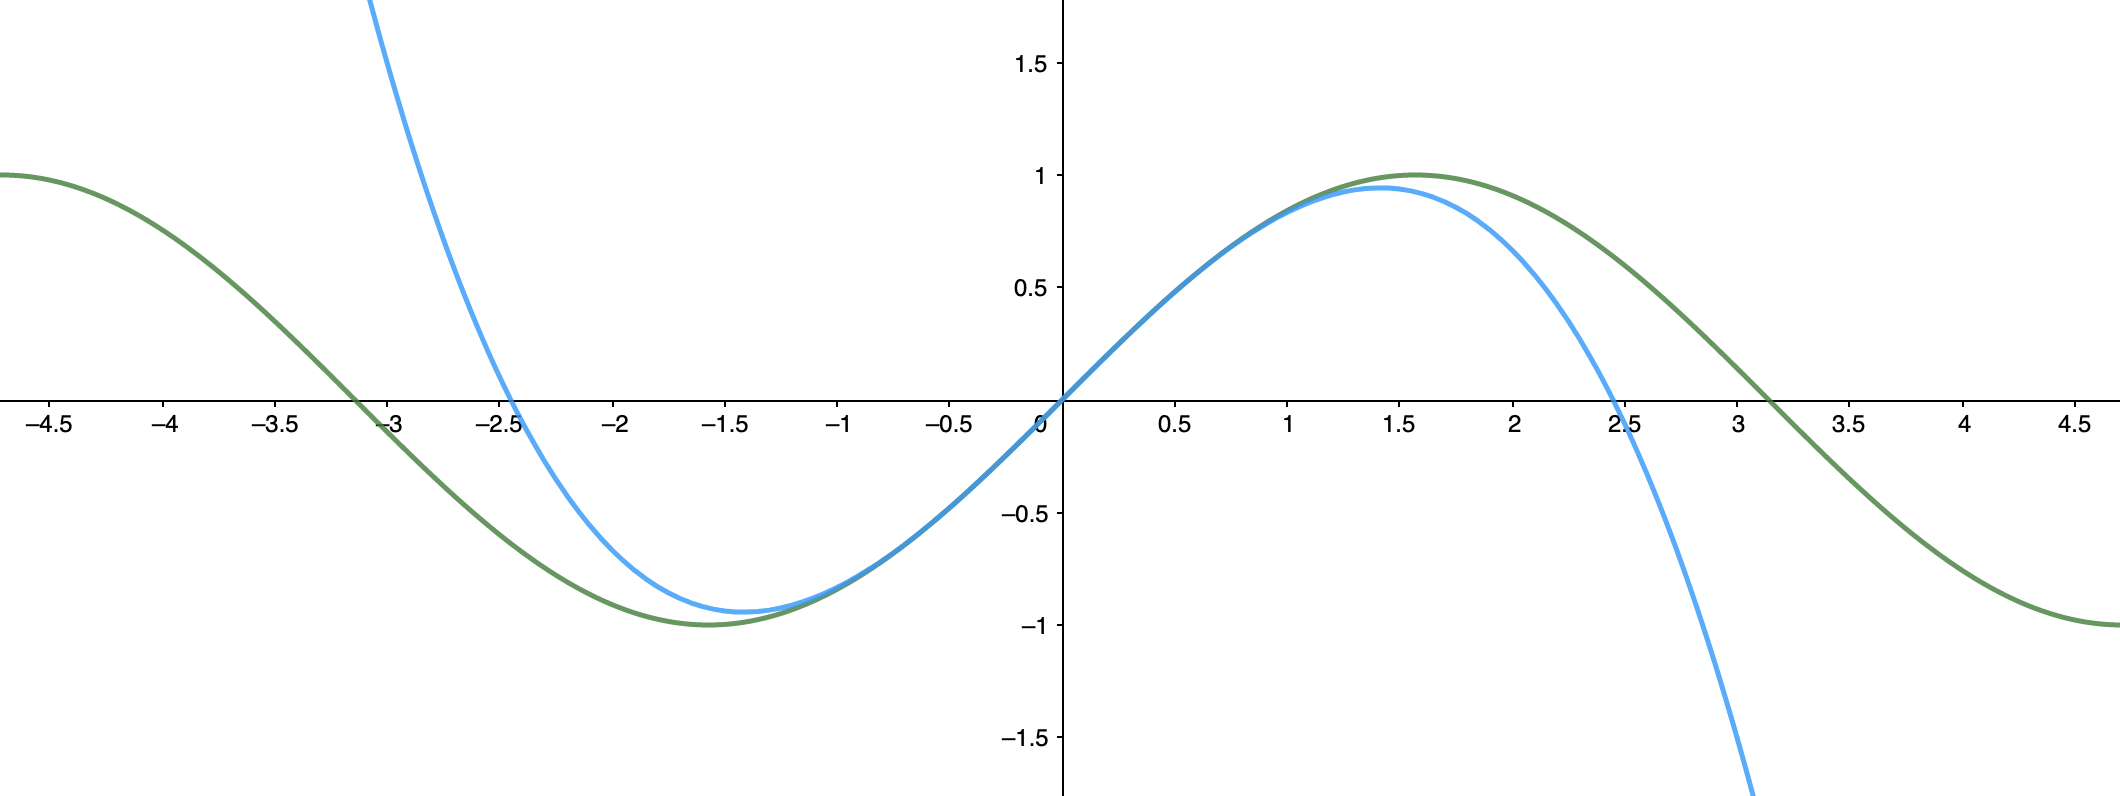
\includegraphics[width=\linewidth]{photos/chapter1/1.png}
    \centerline{Den blåa grafen är $ g(x) $}
\end{figure}
\bigskip

Hur kommer man då fram till detta, och går det att göra bättre approximationer?
\bigskip

I differentialkalkyl så har vi lärt oss att derivator styr formen på grafer av funktioner.
Om derivatan är positiv så kan det visuellt ses som att lutningen är uppåtgående och om andraderivatan är negativ så kan des ses genom att lutningen minskar i samband med att $ x $ ökar.
Om vi har synen av att derivatorna (första, andra, tredje, osv) formar grafen av en funktion så blir fortsättningen lättare.
\bigskip

Vi benämner en polynom i syfte att försöka forma den utefter $ h(x) = \cos x $ nära $ x = 0 $.
\vspace{24pt plus 4pt minus 4pt}

\hspace{5ex}
$ P(x) = a + bx + cx^2 $
\vspace{24pt plus 4pt minus 4pt}

Vi kan styra värdena på $ a $, $ b $ och $ c $ för att ändra formen på grafen av $ P(x) $.
Om vi ser till att $ P(0) = h(0) $, $ P'(0) = h'(0) $, $ P''(0) = h''(0) $, o.s.v. så borde graferna formas liknande runt $ x = 0 $.
Vi börjar med att se vad $ a $ borde vara.
\vspace{24pt plus 4pt minus 4pt}

\hspace{5ex}
$ P(0) = a $

\hspace{5ex}
$ h(0) = cos(0) = 1 $
\bigskip

\hspace{5ex}
$ P(0) = h(0) \iff a = 1 $
\bigskip

\hspace{5ex}
$ P(x) = 1 + \dots $

\begin{figure}[ht!]
    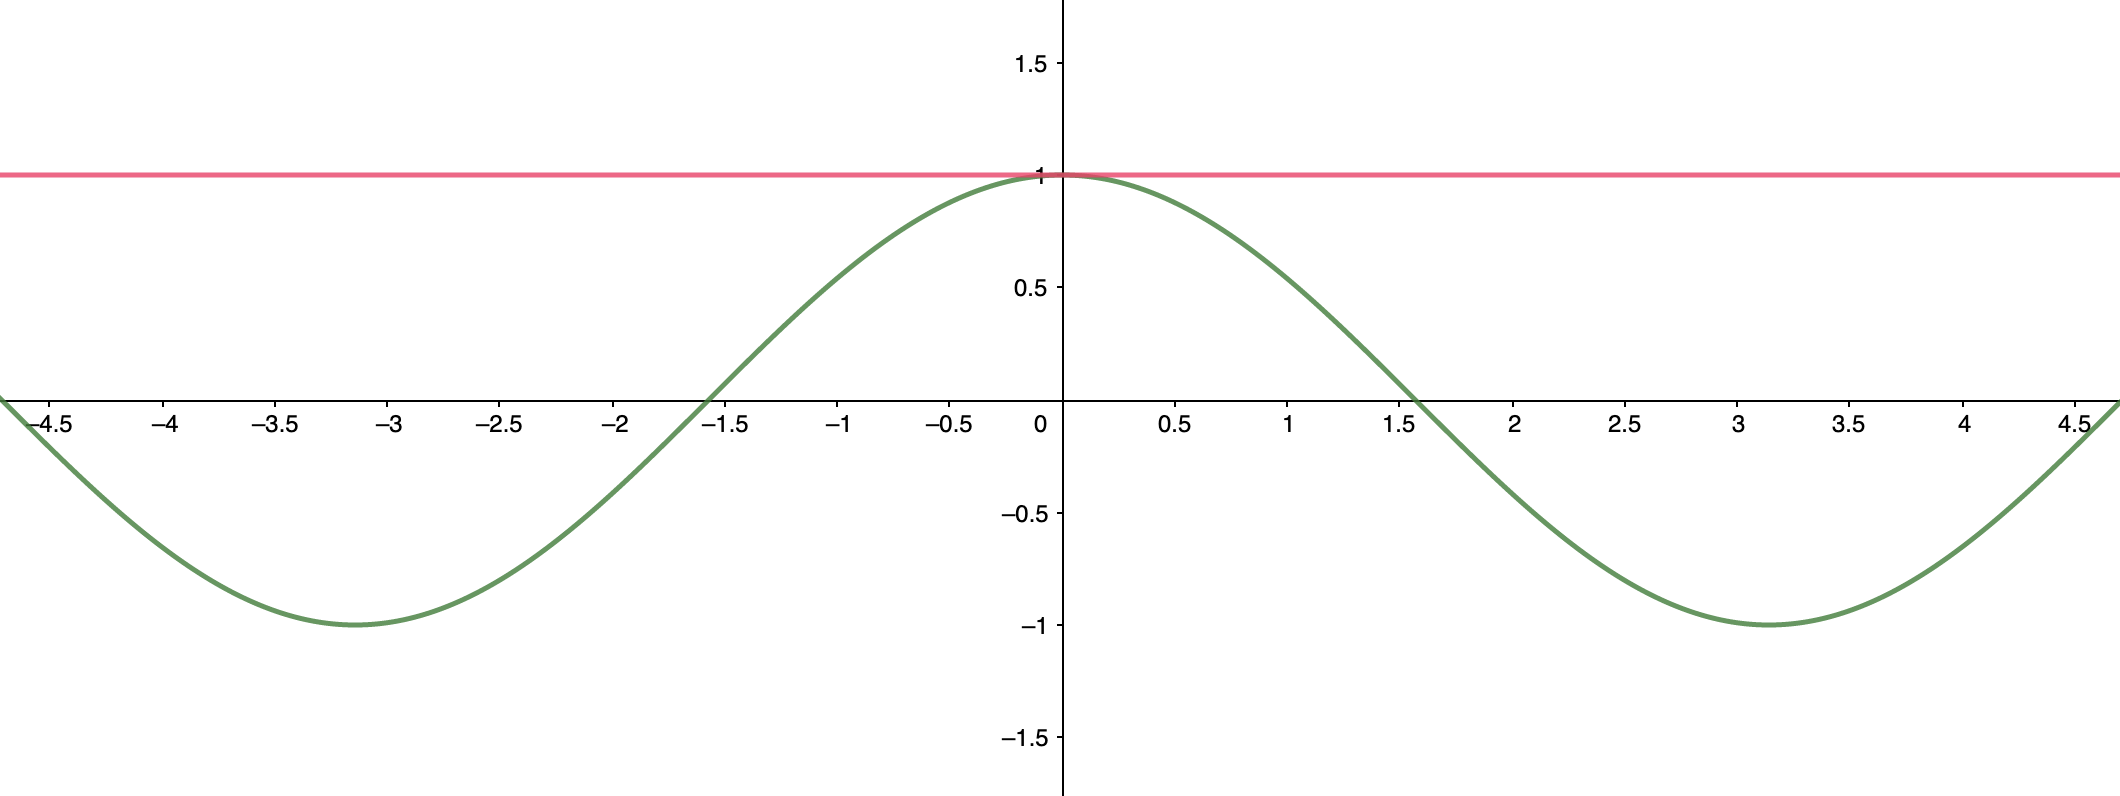
\includegraphics[width=\linewidth]{photos/chapter1/2.png}
    \centerline{Den röda linjen är $ y = 1 $}
\end{figure}
\bigskip

Det är nu rätt självklart att $ a = 1 $, för det betyder att $ P(x) $ korsar $ h(x) $ vid x = 0. 
Vi fortsätter med nästa konstant, b.
\vspace{24pt plus 4pt minus 4pt}

\hspace{5ex}
$ P'(x) = b + 2cx \Rightarrow P'(0) = b $

\hspace{5ex}
$ h'(x) = -\sin x \Rightarrow h'(0) = 0 $
\bigskip

\hspace{5ex}
$ P'(0) = h'(0) \iff b = 0 $
\bigskip

\hspace{5ex}
$ P(x) = 1 + 0x + \dotso = 1 + \dotso $
\vspace{24pt plus 4pt minus 4pt}

Det ändrade inte så mycket, men vi fortsätter med andraderivatan på samma sätt.
\vspace{24pt plus 4pt minus 4pt}

\hspace{5ex}
$ P''(x) = 2c \Rightarrow P''(0) = 2c $

\hspace{5ex}
$ h''(x) = -\cos x \Rightarrow h''(0) = -1 $
\bigskip

\hspace{5ex}
$ P''(0) = h''(0) \iff 2c = -1 \iff c = -\dfrac{1}{2} $
\vspace{24pt plus 4pt minus 4pt}

Detta betyder att;
\vspace{24pt plus 4pt minus 4pt}

\hspace{5ex}
$ a = 1 $

\hspace{5ex}
$ b = 0 $

\hspace{5ex}
$ c = -\dfrac{1}{2} $
\vspace{24pt plus 4pt minus 4pt}

och alltså att;
\vspace{24pt plus 4pt minus 4pt}

\hspace{5ex}
$ P(x) = 1 - \dfrac{1}{2}x^2 $
\bigskip
\bigskip

\begin{figure}[ht!]
    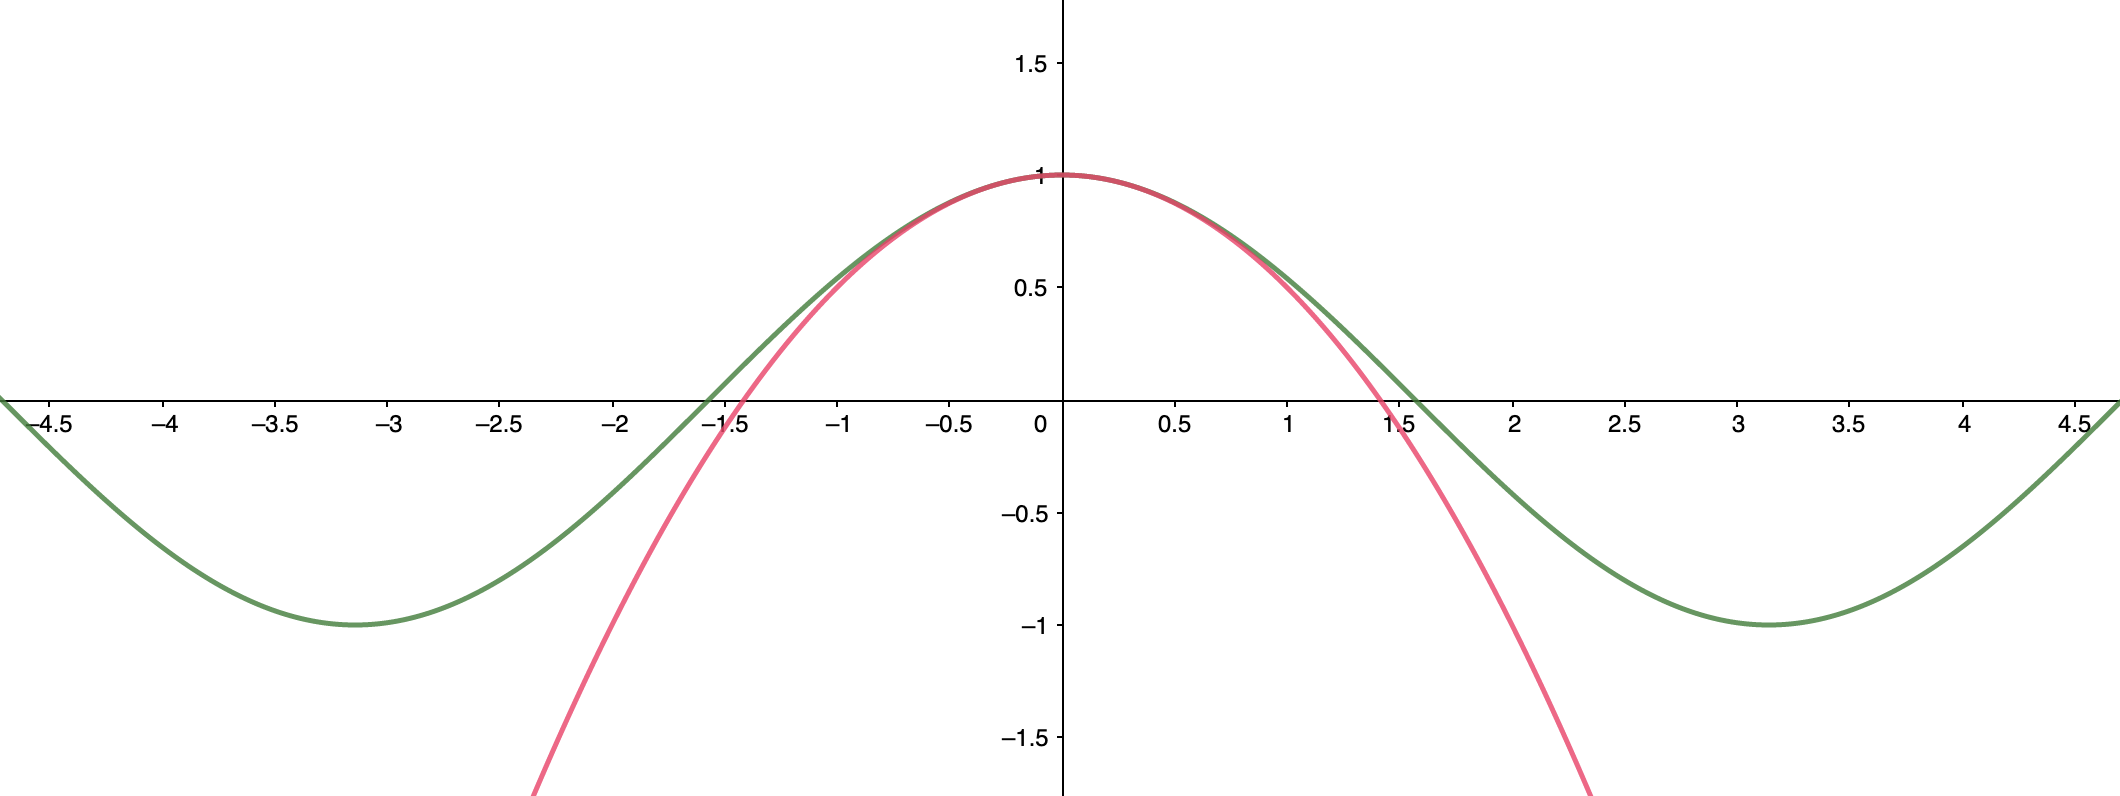
\includegraphics[width=\linewidth]{photos/chapter1/3.png}
    \centerline{Den röda grafen är $ P(x) = 1 - \dfrac{1}{2}x^2 $}
\end{figure}
\bigskip

$ P(x) \approx h(x) $ för val av $ x $ nära $ x = 0 $, vilket var målet.
\bigskip

Nu är såklart frågan; går detta att göra för alla funktioner? Hur gör vi en generell metod? 
För att lösa det så behöver vi se mönstret i vad vi gjorde.
\bigskip

Om vi definierar en polynom $ Q(x) $
\vspace{24pt plus 4pt minus 4pt}

\hspace{5ex}
$ Q(x) = a_0 + a_1x + a_2x^2 + a_3x^3 + \dotso + a_nx^n + a_{n+1}x^{n+1} $
\bigskip
\bigskip

och vi vill skriva konstanten $ a_n $ på ett annat vis, då kan vi få fram konstanten $ a_n $ genom att ta den n:te derivatan $ Q^{(n)}(x) $ som då eliminerar alla termer åt vänster,
och om vi då sätter $ Q^{(n)}(0) $ så elimineras alla termer åt höger som fortfarande är multiplicerade med något antal $ x $. Detta betyder alltså att
\vspace{24pt plus 4pt minus 4pt}

\hspace{5ex}
$ Q^{(n)}(0) = a_n \cdot n! $
\vspace{24pt plus 4pt minus 4pt}

"$ n! $" är där för att vid varje derivering så multipliceras termen med exponenten av $ x $ och för varje derivering så minskar den exponenten med 1 (enligt deriveringsregeln nedan) 
så $ a_n $ multipliceras då med $ n \cdot (n-1) \cdot (n-2) \dotso $ fram tills att $ (n - k) = 1 $,
vilket är samma sak som att säga att $ a_n $ multipliceras med $ n! $ enligt definitionen av fakultet;
\vspace{24pt plus 4pt minus 4pt}

\hspace{5ex}
$ f(x) = ax^n $

\hspace{5ex}
$ f'(x) = anx^{n-1} $

\hspace{5ex}
$ f''(x) = an(n-1)x^{n-2} $

\hspace{5ex}
$ f''(x) = an(n-1)(n-2)x^{n-3} $

\hspace{5ex}
$ f'''(x) = an(n-1)(n-2)(n-3)x^{n-4} $

\hspace{5ex}
$ \dotso $
\vspace{24pt plus 4pt minus 4pt}

Om vi då fortsätter med $ Q(x) $;
\vspace{24pt plus 4pt minus 4pt}

\hspace{5ex}
$ Q^{(n)}(0) = a_n \cdot n! \iff a_n = \dfrac{Q^{(n)}(0)}{n!} $ 
\vspace{24pt plus 4pt minus 4pt}

Vilket betyder att;
\vspace{24pt plus 4pt minus 4pt}

\hspace{5ex}
$ Q(x) = a_0 + a_1x + a_2x^2 + a_3x^3 + \dotso + a_nx^n + a_{n+1}x^{n+1} $
\bigskip

\hspace{10ex}
$ \Updownarrow $
\bigskip

\hspace{5ex}
$ Q(x) = \dfrac{Q^{(0)}(0)}{0!} + \dfrac{Q^{(1)}(0)}{1!}x + \dfrac{Q^{(2)}(0)}{2!}x^2 + \dfrac{Q^{(3)}(0)}{3!}x^3 + \dotso + \dfrac{Q^{(n)}(0)}{n!}x^n + \dfrac{Q^{(n+1)}(0)}{(n+1)!}x^{n+1} $ 
\vspace{24pt plus 4pt minus 4pt}

och ett snyggare sätt att skriva detta på är;
\vspace{24pt plus 4pt minus 4pt}

\hspace{5ex}
$ Q(x) = \sum\limits_{k=0}^{n} \dfrac{Q^{k}(0)}{k!}x^k $ 
\vspace{24pt plus 4pt minus 4pt}

Nu är vi snart vid Maclaurinserien i sin fullhet. 
Om vi definierar en oändlig polynom;
\vspace{24pt plus 4pt minus 4pt}

\hspace{5ex}
$ f(x) = a_0 + a_1x + a_2x^2 + a_3x^3 + \dotso $
\vspace{24pt plus 4pt minus 4pt}

Så kan vi skriva den som;
\vspace{24pt plus 4pt minus 4pt}

\hspace{5ex}
$ f(x) = \sum\limits_{k=0}^{\infty} \dfrac{Q^{(k)}(0)}{k!}x^k $ 
\vspace{24pt plus 4pt minus 4pt}

vilket är Maclaurinserien av $ f(x) $.
\bigskip

Det som är praktiskt med denna serie är att vi kan använda den till att skriva icke-polynomfunktioner till formen av en polynom.
För icke-polynomfunktioner som har ett mönster i hur derivatorna ser ut så kan vi faktiskt skapa en oändlig polynom som är lika med den funktionen,
med hjälp av maclaurinserien. Vi testar $ h(x) = \cos x $ från tidigare, som exempel. Derivatorna av $ \cos x $ följer ett tydligt mönster;
\vspace{24pt plus 4pt minus 4pt}

\hspace{5ex}
$ h(x) = \cos x $

\hspace{5ex}
$ h^{(1)}(x) = -\sin x $

\hspace{5ex}
$ h^{(2)}(x) = -\cos x $

\hspace{5ex}
$ h^{(3)}(x) = \sin x $

\hspace{5ex}
$ h^{(4)}(x) = \cos x $

\hspace{5ex}
$ \dotso $
\vspace{24pt plus 4pt minus 4pt}

vilket betyder att;
\vspace{24pt plus 4pt minus 4pt}

\hspace{5ex}
$ h(0) = 1 $

\hspace{5ex}
$ h^{(1)}(0) = 0 $

\hspace{5ex}
$ h^{(2)}(0) = -1 $

\hspace{5ex}
$ h^{(3)}(0) = 0 $

\hspace{5ex}
$ h^{(4)}(0) = 1 $

\hspace{5ex}
$ \dotso $
\vspace{24pt plus 4pt minus 4pt}

och alltså att;
\vspace{24pt plus 4pt minus 4pt}

\hspace{5ex}
$ f(x) = \sum\limits_{k=0}^{\infty} \dfrac{Q^{(k)}(0)}{k!}x^k $ 
\bigskip

\hspace{10ex}
$ \Downarrow $
\bigskip

\hspace{5ex}
$ h(x) = \dfrac{h^{(0)}(0)}{0!} + \dfrac{h^{(1)}(0)}{1!}x + \dfrac{h^{(2)}(0)}{2!}x^2 + \dfrac{h^{(3)}(0)}{3!}x^3 + \dfrac{h^{(4)}(0)}{4!}x^4 + \dotso $
\bigskip

\hspace{10ex}
$ \Downarrow $
\bigskip

\hspace{5ex}
$ h(x) = \dfrac{1}{0!} + \dfrac{0}{1!}x + \dfrac{-1}{2!}x^2 + \dfrac{0}{3!}x^3 + \dfrac{1}{4!}x^4 + \dotso $ 
\bigskip

\hspace{10ex}
$ \Downarrow $
\bigskip

\hspace{5ex}
$ h(x) = 1 - \dfrac{1}{2!}x^2 + \dfrac{1}{4!}x^4 + \dotso $ 
\bigskip

\hspace{10ex}
$ \Updownarrow $
\bigskip

\hspace{5ex}
$ h(x) = \sum\limits_{k=0}^{\infty} \dfrac{(-1)^k}{(2k)!}x^k $
\bigskip

\hspace{10ex}
$ \Downarrow $
\bigskip

\hspace{5ex}
$ \cos x = \sum\limits_{k=0}^{\infty} \dfrac{(-1)^k}{(2k)!}x^{2k} $
\vspace{24pt plus 4pt minus 4pt}

Om vi nu testar att ta de första fem termerna utefter denna serie och ser hur den approximerar $ \cos x $ så kan vi se att det definitivt fungerar;

\begin{figure}[ht!]
    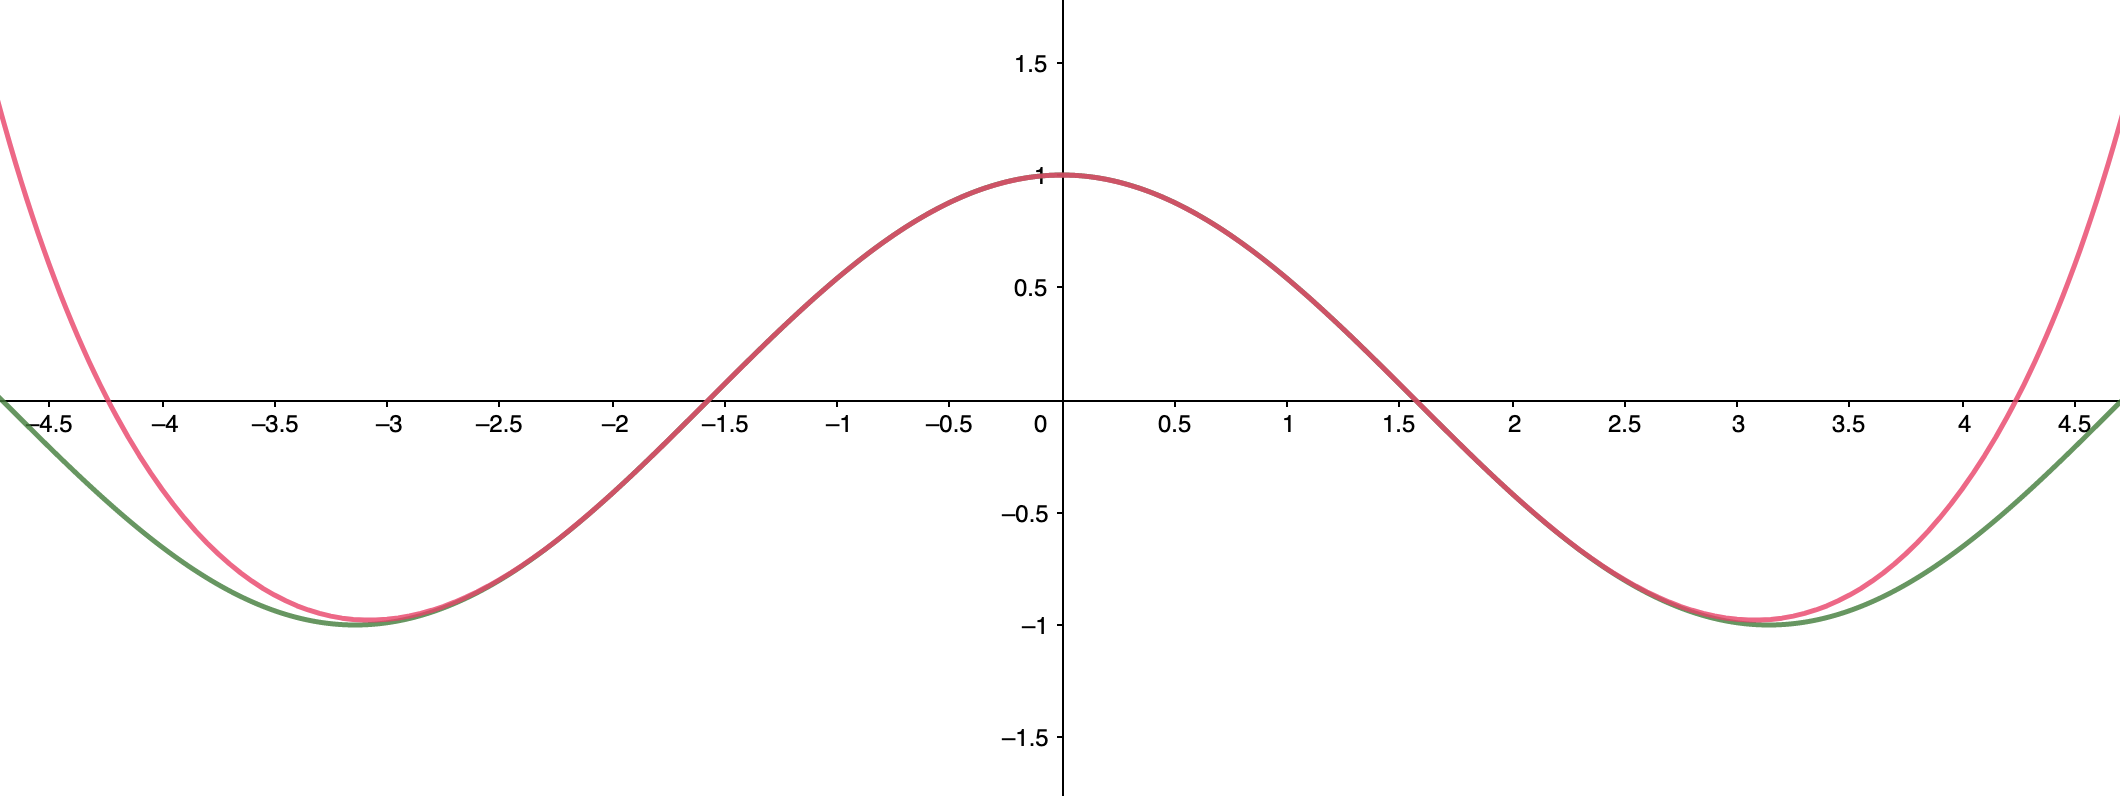
\includegraphics[width=\linewidth]{photos/chapter1/4.png}
    \centerline{Den röda grafen är $ y = 1 - \dfrac{1}{2!}x^2 + \dfrac{1}{4!}x^4 - \dfrac{1}{6!}x^6 + \dfrac{1}{8}x^8$}
\end{figure}
\bigskip

Detta kapitel nämner också en så kallad "Taylorserie", så vad är det då? Det är en mer generell Maclaurinserie som kan jämföra derivatorna runt $ x = a $ istället för $ x = 0 $,
vilket är användbart ifall man behöver approximera en funktion runt ett annat värde än just $ x = 0 $. Vi kan bygga oss fram till definitionen på ett liknande sätt:
\bigskip

Vi definierar en oändlig polynom;
\bigskip

\bigskip
\hspace{5ex}
$ f(x) = a_0(x-a)^0 + a_1(x-a)^1 + a_2(x-a)^2 + \dotso $
\vspace{24pt plus 4pt minus 4pt}

Anledningen varför vi har faktorer av $ (x - a) $ är att vi vill kunna eliminera alla termer åt höger om någon konstant efter en viss mängd deriveringar, 
genom att evaluera den derivatan av polynomen vid $ x = a $, och inte vid $ x = 0 $, som vi gjorde för Maclaurinserien. 
Detta gör att vi kan bygga serien med information vid $ x = a $ istället för vid $ x = 0 $, 
vilket kommer att leda till att när vi väljer ett ändligt antal termer från den oändliga serien för att skapa en approximation av en icke-polynom så kommer den att approximera bäst runt $ x = a $ istället för $ x = 0 $.

\begin{figure}[ht!]
    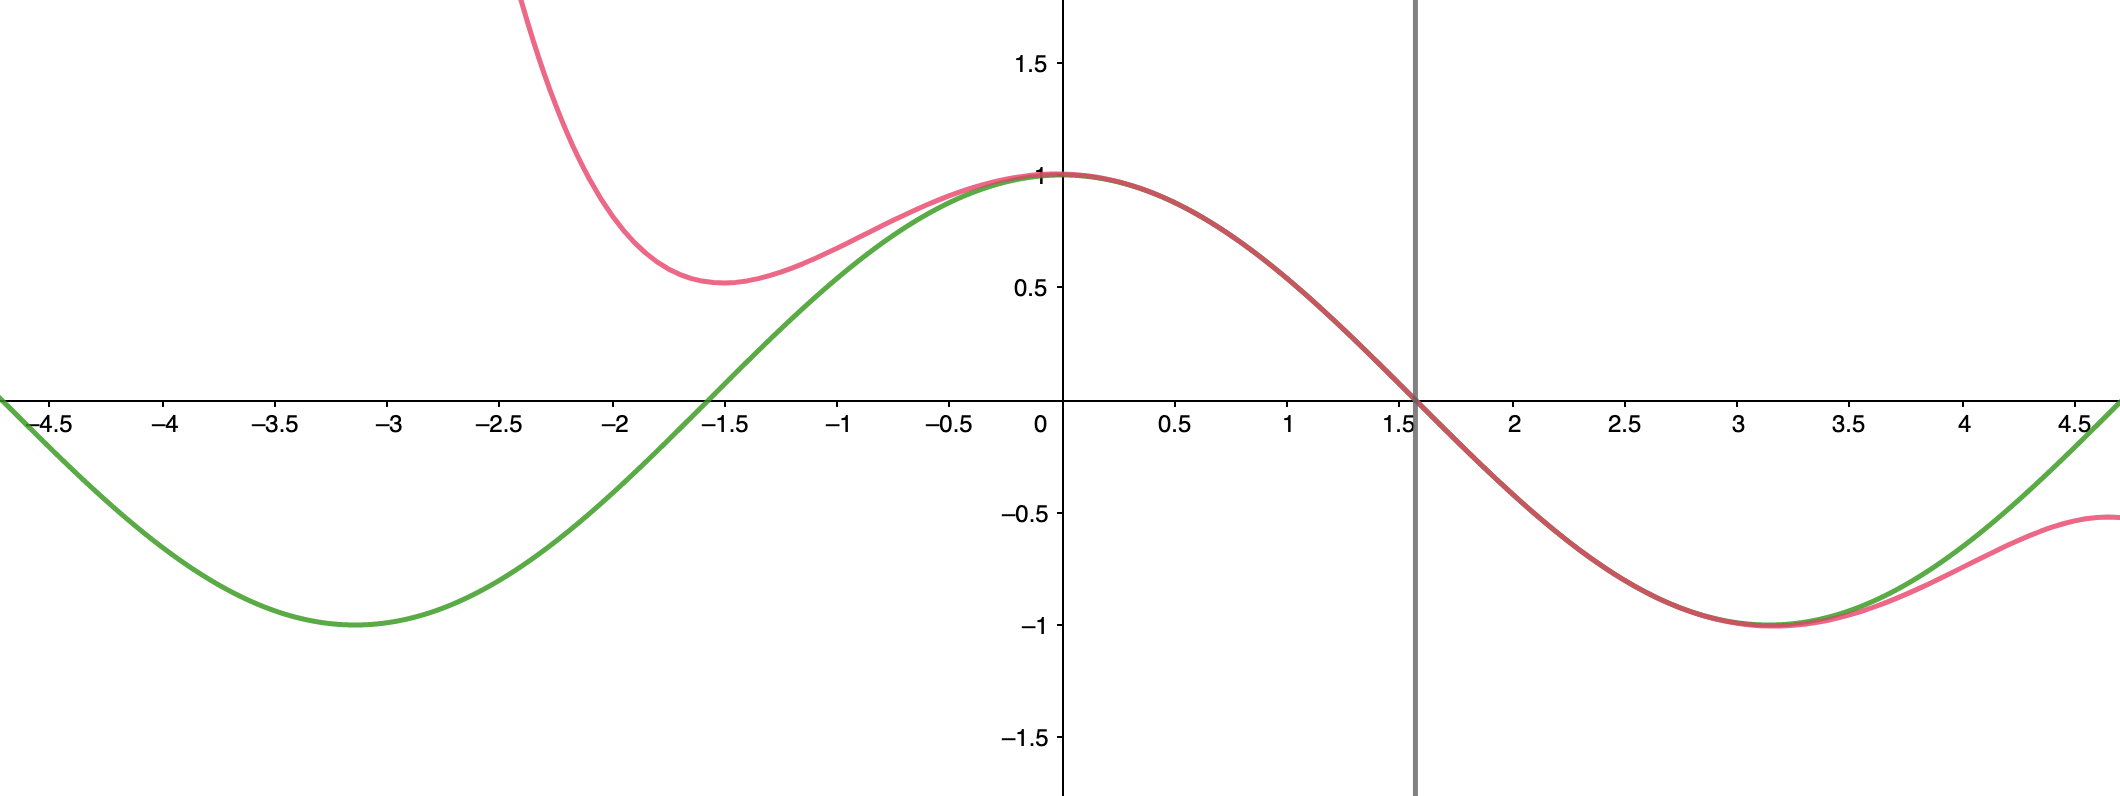
\includegraphics[width=\linewidth]{photos/chapter1/5.png}
    \centerline{taylorapproximering av $ \cos x $ med fyra termer, evaluerad vid $ x = \dfrac{\pi}{2} $}
\end{figure}
\bigskip

Med den förståelsen så kan vi fortsätta med polynomen $ f(x) $. Med samma argument som tidigare så ska detta stämma;
\vspace{24pt plus 4pt minus 4pt}

\bigskip
\hspace{5ex}
$ f^{(n)}(a) = a_n \cdot n! \iff a_n = \dfrac{f^{(n)}(a)}{n!} $ 
\vspace{24pt plus 4pt minus 4pt}

Vilket betyder att;
\vspace{24pt plus 4pt minus 4pt}

\hspace{5ex}
$ f(x) = a_0(x-a)^0 + a_1(x-a)^1 + a_2(x-a)^2 + \dotso $
\bigskip 

\hspace{10ex}
$ \Updownarrow $
\bigskip

\hspace{5ex}
$ f(x) = \dfrac{f^{(0)}(a)}{0!}(x-a)^0 + \dfrac{f^{(1)}(a)}{1!}(x-a)^1 + \dfrac{f^{(2)}(a)}{2!}(x-a)^2 + \dotso $
\bigskip

\hspace{10ex}
$ \Updownarrow $
\bigskip

\hspace{5ex}
$ f(x) = \sum\limits_{k=0}^{\infty} \dfrac{f^{(k)}(a)}{k!}(x-a)^k $ 
\vspace{24pt plus 4pt minus 4pt}

Vilket är Taylorserien i sin fullhet. I detta kapitel så har jag har valt att visualisera detta med hjälp av trigonometriska funktioner men detta kan självklart användas till att approximera exponentiella funktioner, logaritmiska funktioner och till och med komplexa funktioner (checka $ e^{ix} $ om du är nyfiken!).
En viktig sak att nämna är att en taylorserie inte finns för alla funktioner. En funktion måste vara analytisk för att ha en ekvivalent taylorserie. 
Ett exempel som inte har någon taylorserie är $ s(x) = \abs{x} $, för $ s(x) $ är inte deriverbar vid $ x = 0 $.

% ------------------------------------------------------------------------------------------------------------------------------------------------------------------------
\newpage
\section{Eulers formel}
\bigskip

I detta kapitel så kommer jag anta förståelse av grunderna inom komplexa tal, och då menar jag hantering av addition och multiplikation och vad det resulterar i visuellt sett.
\bigskip

Många har nog sett denna formel någon gång, Eulers formel;
\vspace{24pt plus 4pt minus 4pt}

\hspace{5ex}
$ e^{ix} = \cos x + i\sin x $
\bigskip
\bigskip

Det är ganska lätt att visa att det stämmer, rent algebraiskt, med hjälp av macluarinserierna av $ e^x $, $ \cos x $ och $ \sin x $ (som vi har gått igenom i ett av de andra kapitlena);
\vspace{24pt plus 4pt minus 4pt}

\hspace{5ex}
$ e^x = 1 + x + \dfrac{x^2}{2!} + \dfrac{x^3}{3!} + \dfrac{x^4}{4!} + \dotso $
\bigskip

\hspace{10ex}
$ \Updownarrow $
\bigskip

\hspace{5ex}
$ e^{ix} = 1 + (ix) + \dfrac{(ix)^2}{2!} + \dfrac{(ix)^3}{3!} + \dfrac{(ix)^4}{4!} + \dotso $
\bigskip

\hspace{10ex}
$ \Updownarrow $
\bigskip

\hspace{5ex}
$ e^{ix} = 1 + ix - \dfrac{x^2}{2!} - i\dfrac{x^3}{3!} + \dfrac{x^4}{4!} + \dotso $
\vspace{24pt plus 4pt minus 4pt} 

och;
\bigskip

\bigskip
\hspace{5ex}
$ \cos x = 1 - \dfrac{x^2}{2!} + \dfrac{x^4}{4!} - \dfrac{x^6}{6!} + \dfrac{x^8}{8!} + \dotso $
\bigskip

och;
\vspace{24pt plus 4pt minus 4pt} 

\hspace{5ex}
$ \sin x = x - \dfrac{x^3}{3!} + \dfrac{x^5}{5!} - \dfrac{x^7}{7!} + \dfrac{x^9}{9!} + \dotso $
\bigskip

\hspace{10ex}
$ \Updownarrow $
\bigskip

\hspace{5ex}
$ i\sin x = ix - i\dfrac{x^3}{3!} + i\dfrac{x^5}{5!} - i\dfrac{x^7}{7!} + i\dfrac{x^9}{9!} + \dotso $
\bigskip
\bigskip

och om vi nu delar upp $ e^{ix} $ i två delar och jämför med $ \cos x + i\sin x $ så kan vi se att formeln stämmer;
\bigskip

\bigskip
\hspace{5ex}
$ e^{ix} = 1 + ix - \dfrac{x^2}{2!} - i\dfrac{x^3}{3!} + \dfrac{x^4}{4!} + i\dfrac{x^5}{5!} + \dotso $
\bigskip

\hspace{10ex}
$ \Updownarrow $
\bigskip

\hspace{5ex}
$ e^{ix} = \left(1 - \dfrac{x^2}{2!} + \dfrac{x^4}{4!} + \dotso\right) + \left(ix - i\dfrac{x^3}{3!} + i\dfrac{x^5}{5!} + \dotso\right) $
\bigskip

\hspace{10ex}
$ \Updownarrow $
\bigskip

\hspace{5ex}
$ e^{ix} = \cos x + i\sin x $
\bigskip
\bigskip

Formeln är alltså tydligt korrekt, men detta ger (för mig iallafall) ingen insikt i varför det borde stämma, mer än att siffrorna bara hänger ihop.
Jag ska nu försöka ge en alternativ förklaring som inte är ett bevis, men som ger en mer visuell förståelse av formeln.
\bigskip

Vi börjar med en av de första frågorna som kan upptså upp när man tittar på eulers formel, vad betyder det ens att ha en imaginär exponent?
Ett sätt att se på det är att se vad som händer när vi deriverar ett uttryck med en imaginär exponent;
\bigskip

\bigskip
\hspace{5ex}
$ f(x) = 2^{ix} $

\hspace{10ex}
$ \Downarrow $

\hspace{5ex}
$ f'(x) = i \cdot \log(2) \cdot 2^{ix} $
\bigskip
\bigskip

Om vi nu sätter in $ x = 0 $;
\bigskip

\bigskip
\hspace{5ex}
$ f(0) = 2^{0i} = 1 $

\hspace{5ex}
$ f'(0) = i \cdot \log(2) \cdot 2^{0i} = i \cdot \log(2) \cdot f(0) $
\bigskip
\bigskip

så kan vi visualisera det såhär i det komplexa talplanet om vi tänker på funktionen och dess derivata som pilar;
\bigskip

\bigskip
\hspace{5ex}
den gröna pilens ände: $ f(0) $

\hspace{5ex}
den röda pilen: $ f'(0) = i \cdot \log(2) \cdot f(0) \approx i \cdot 0.69 \cdot f(0) $

\bigskip
\begin{figure}[H]
    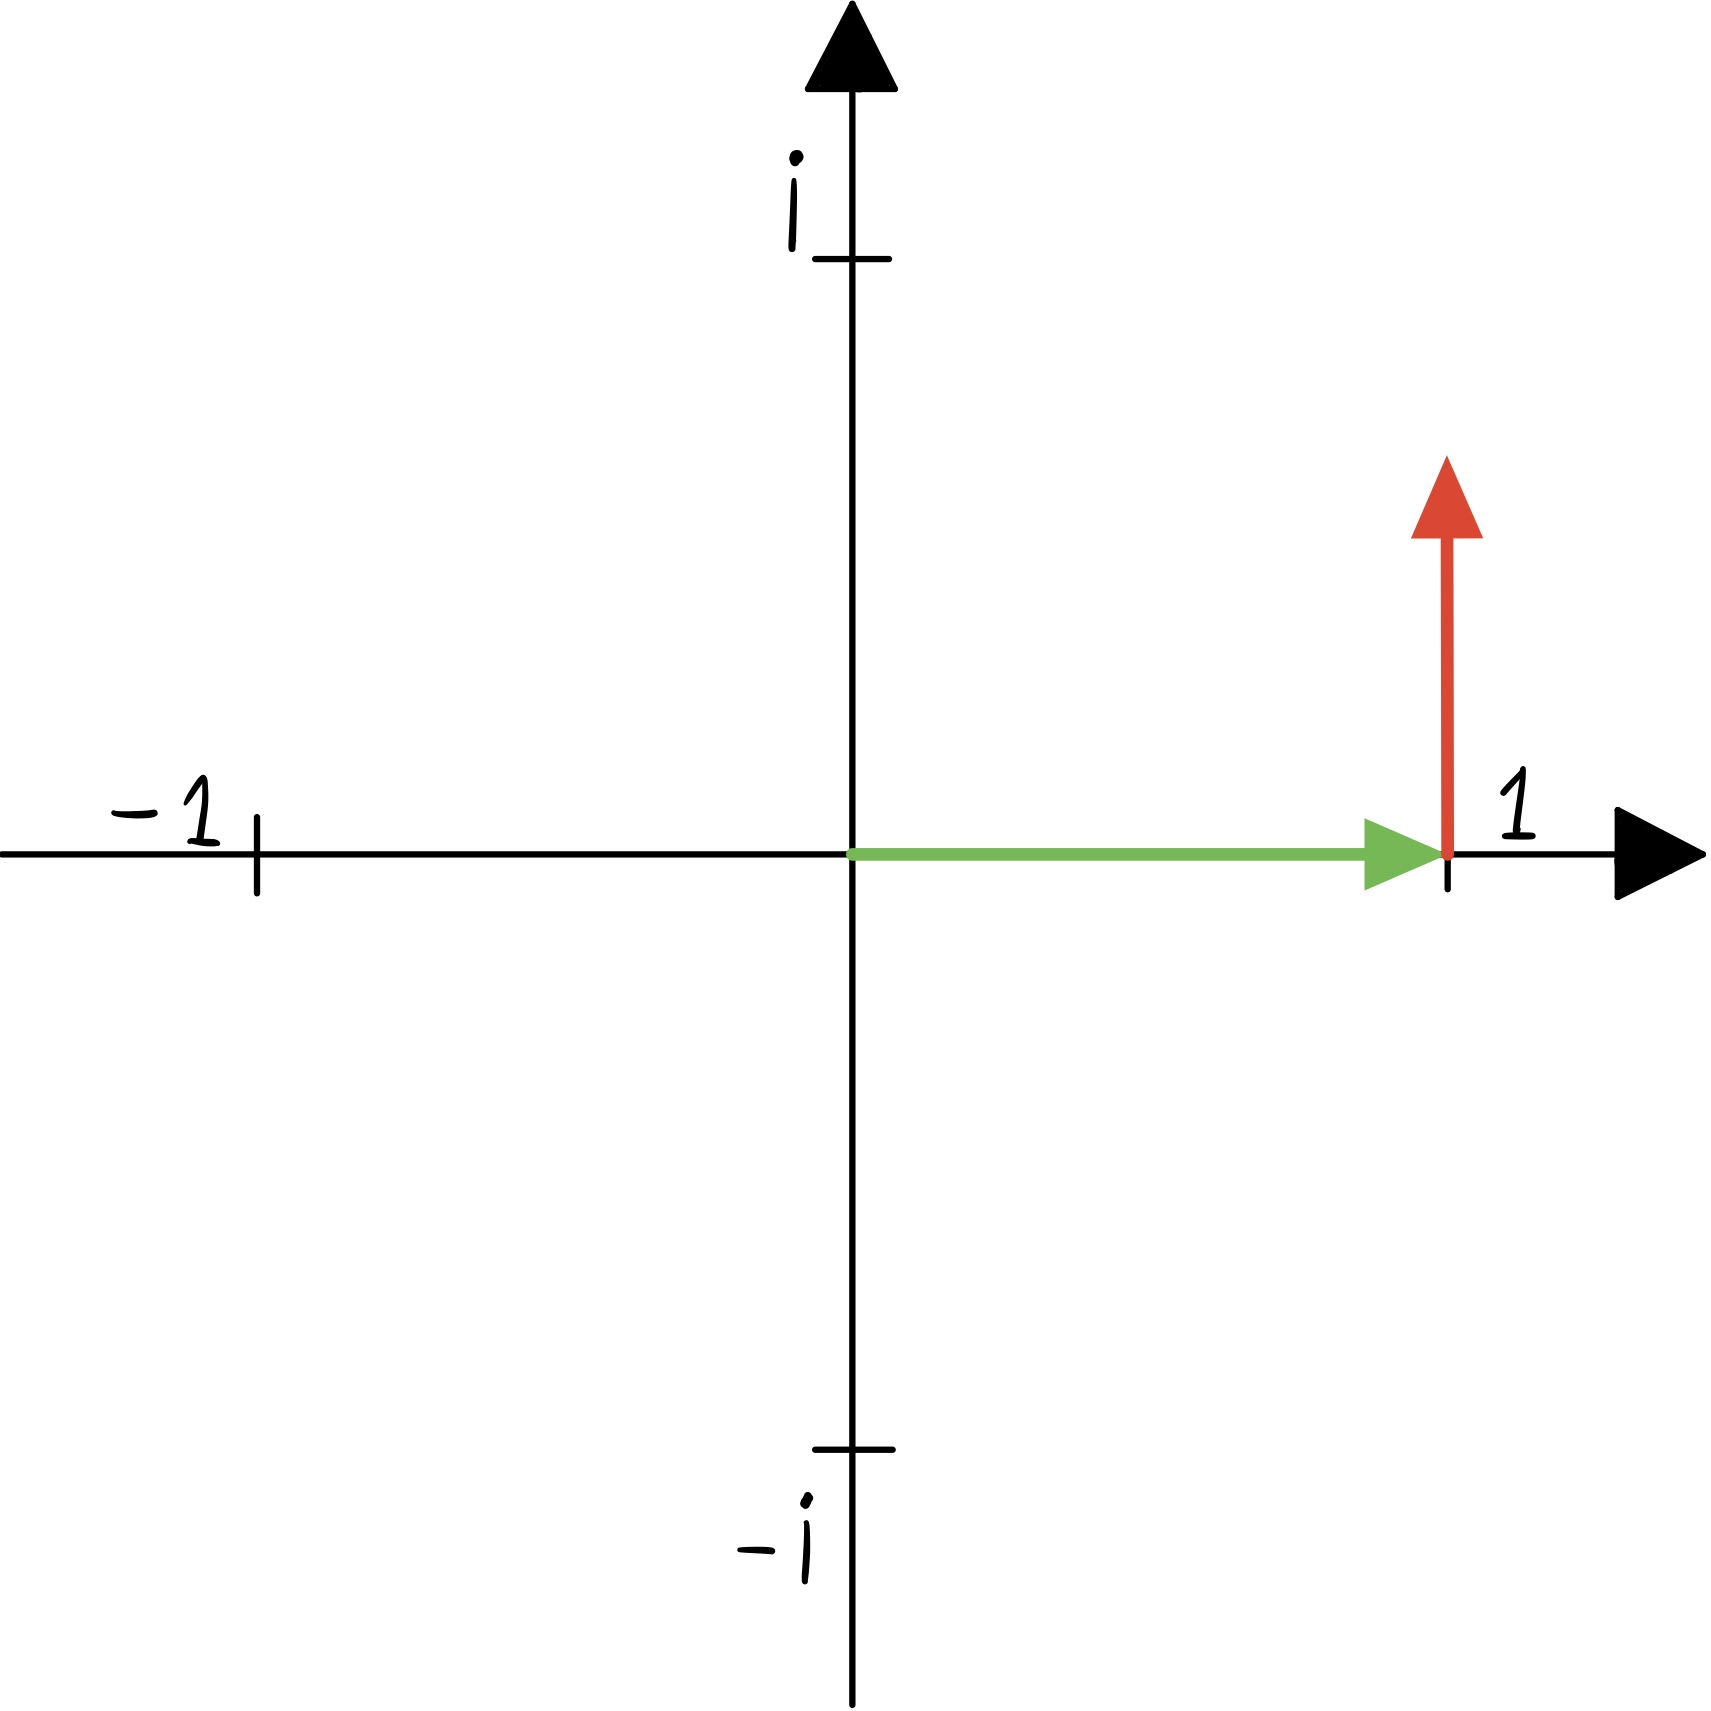
\includegraphics[width=50ex]{photos/chapter2/1.jpg}
\end{figure}

För att den röda pilen är $ \approx i \cdot 0.69 \cdot f(0) $ så är det rimligt att den ser ut som den gröna pilen fast med en 90 graders rotering åt vänster och med förkortad längd.
Detta faktum gäller för alla $ x $ och inte bara för $ x = 0 $. Vad det betyder är att förändringshastigheten av $ f(x) $ alltid är vinkelrät mot (och i detta fallet också nedskalad i storlek) $ f(x) $.
Den viktiga slutsatsen utifrån detta är att om vi låter $ x $ gå från $ 0 $ till något annat värde så kommer inte den gröna pilen att bli längre eller kortare, då förändringshastigheten är vinkelrät.
Det som istället sker är att ändan av den gröna pilen ritar ut en cirkel när $ x $ ökar just för att förändringshastigheten alltid är vinkelrät mot positionen;
\bigskip

\bigskip
\hspace{5ex}
den gröna pilens ände: $ f(x) $

\hspace{5ex}
den röda pilen: $ f'(x) \approx i \cdot 0.69 \cdot f(x) $

\begin{figure}[H]
    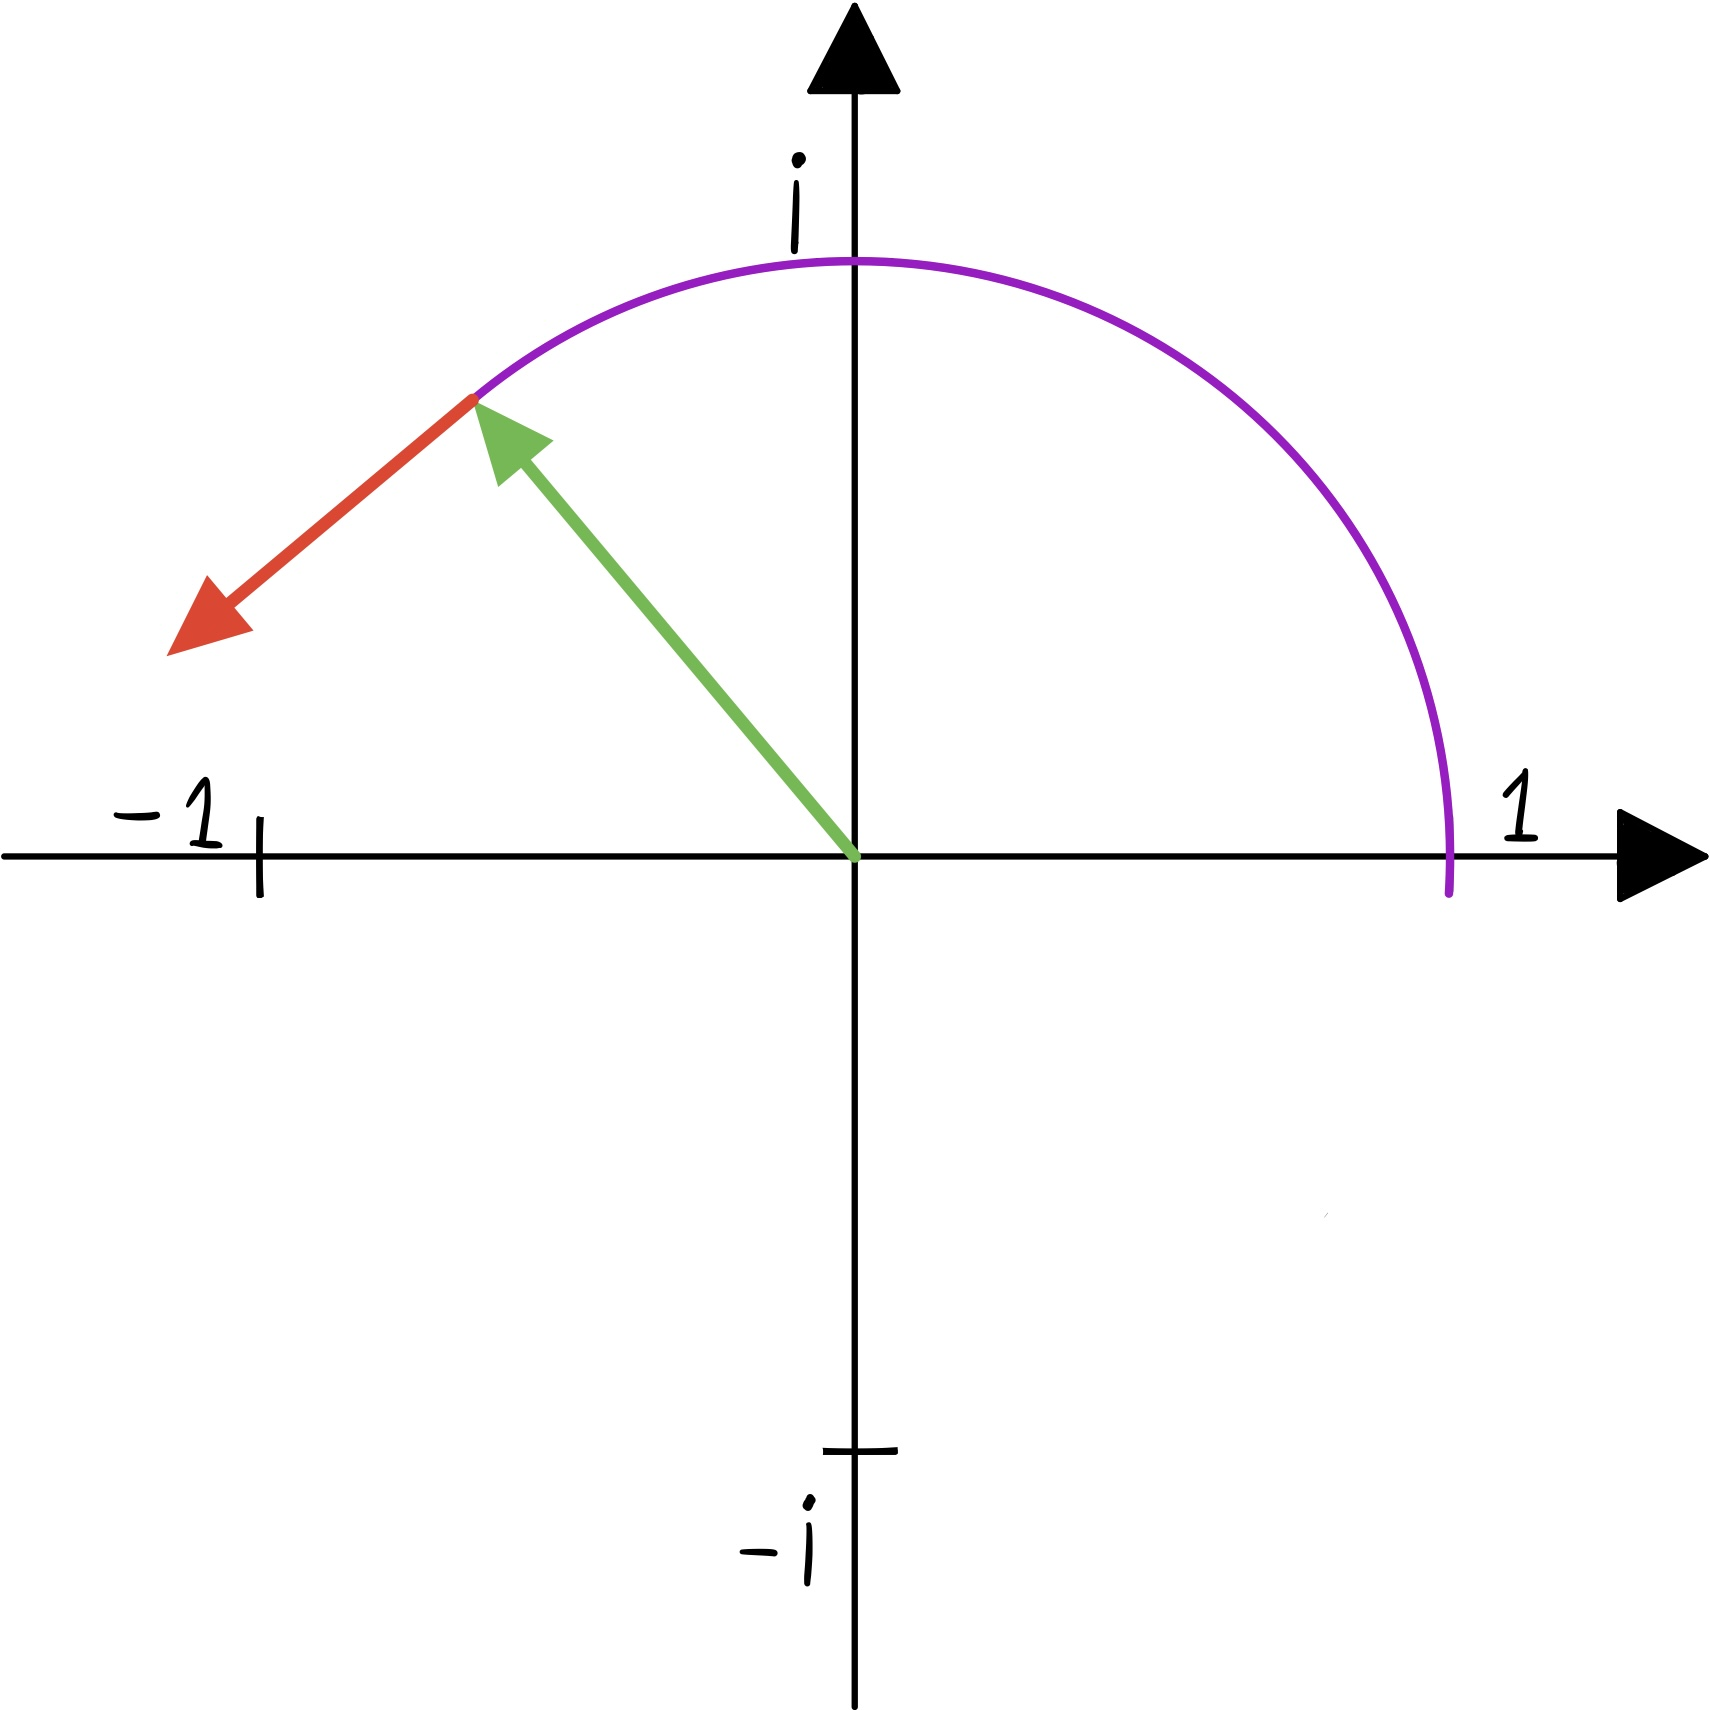
\includegraphics[width=50ex]{photos/chapter2/2.jpg}
\end{figure}

\begin{figure}[H]
    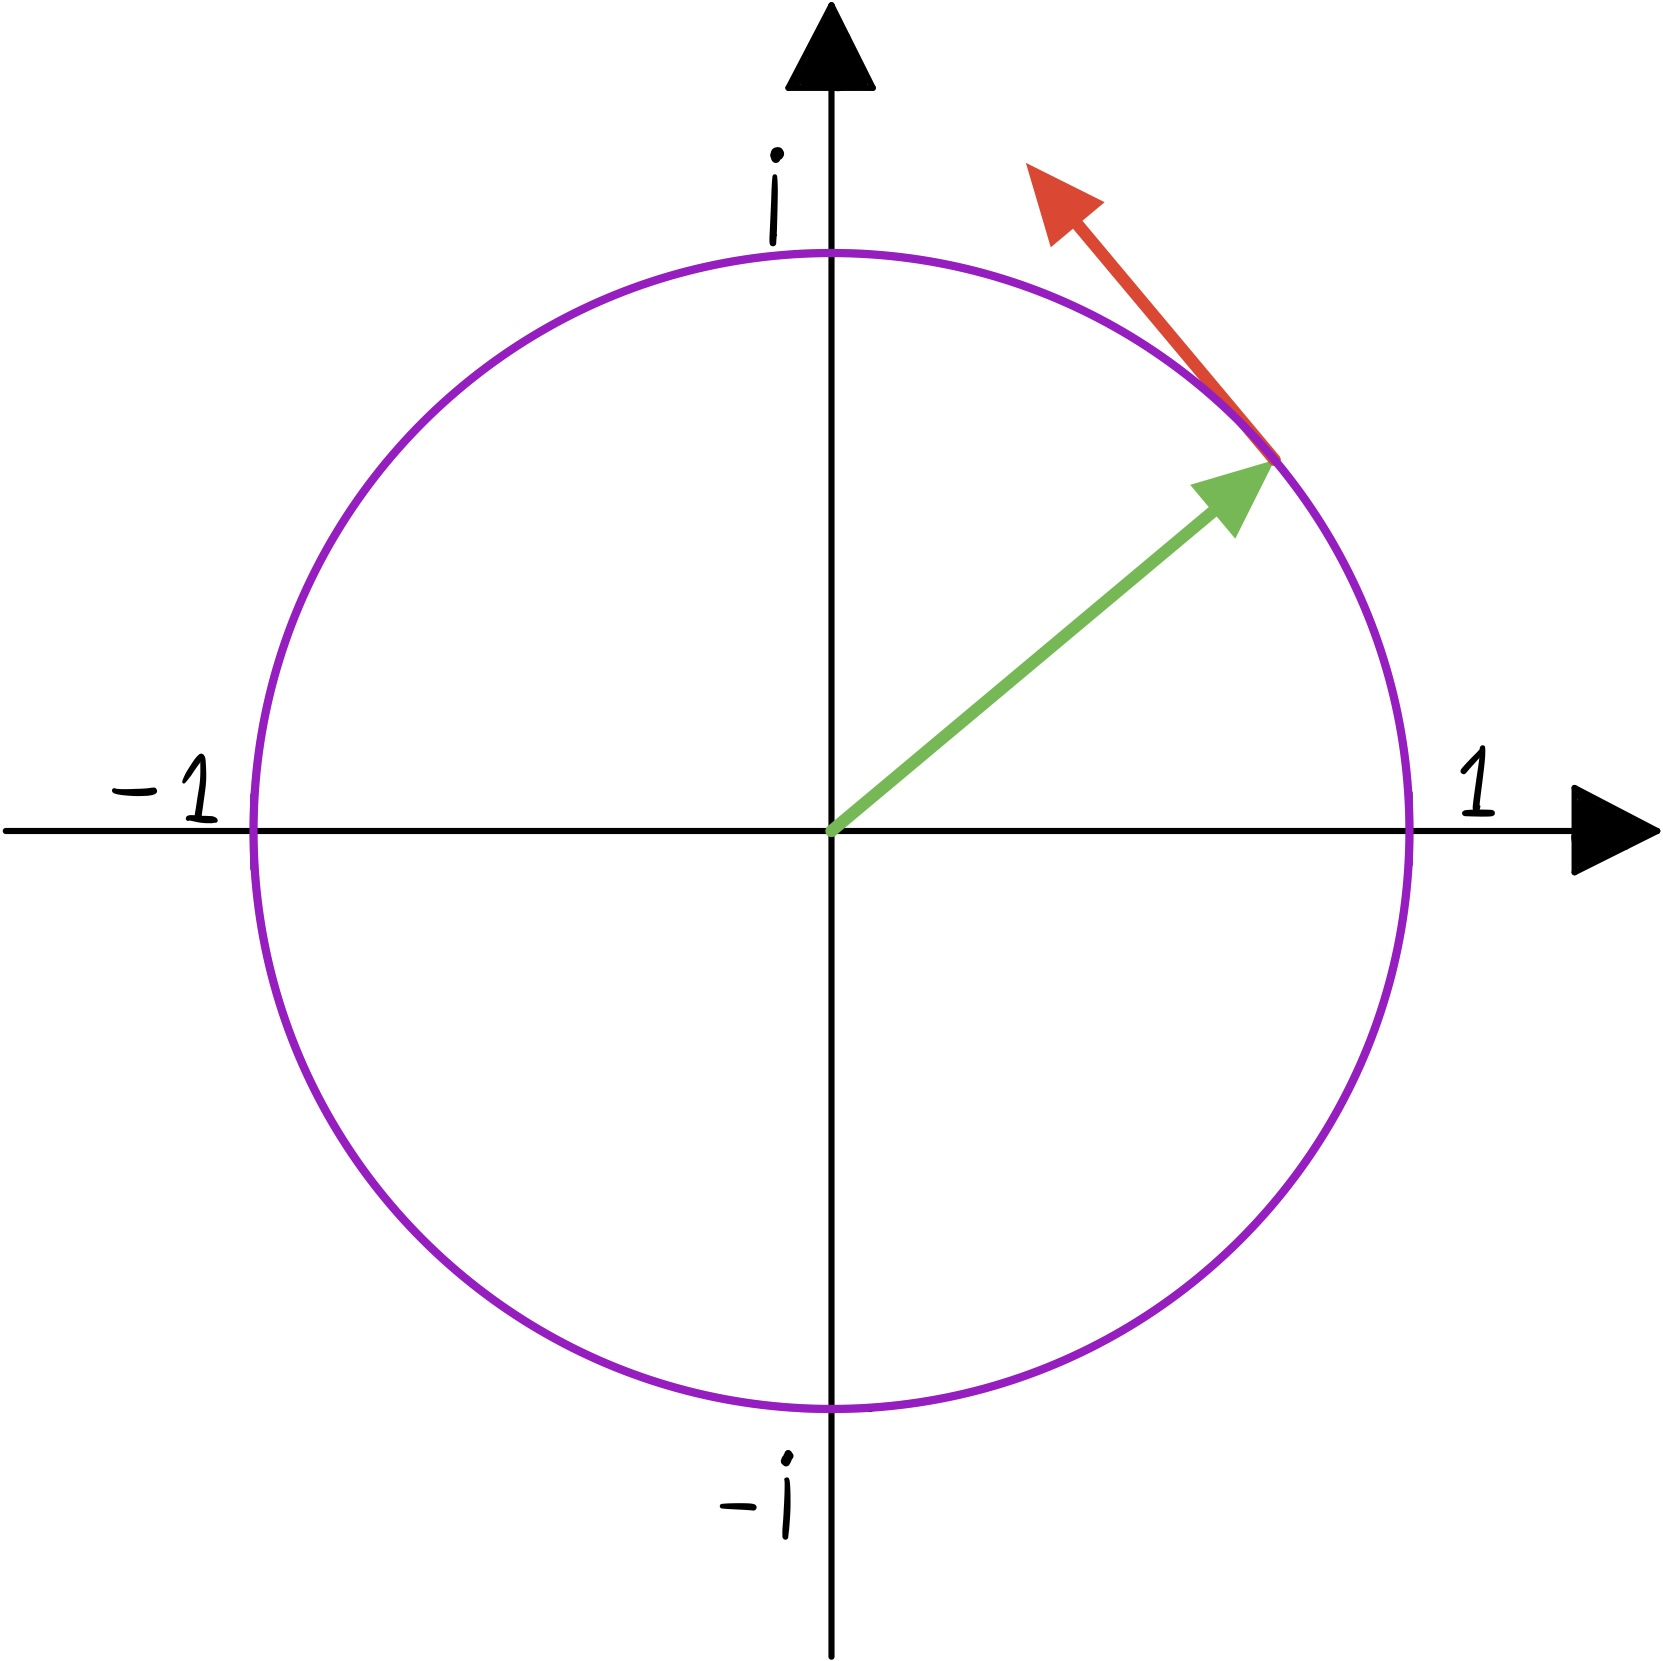
\includegraphics[width=50ex]{photos/chapter2/3.jpg}
\end{figure}

Nu kanske du börjar se att det finns något slags samband mellan imaginära exponenter och trigonometriska uttryck, om du har sett enhetscirkeln innan. Om vi nu övergår till att använda $ f(x) = e^{ix} $ istället för $ f(x) = 2^{ix} $ så får vi lite nya användbara egenskaper;
\bigskip

\bigskip
\hspace{5ex}
$ f(x) = e^{xi} $

\hspace{5ex}
$ f'(x) = i \cdot e^{xi} = i \cdot f(x) $ 
\bigskip
\bigskip

Detta betyder att förändringshastigheten har exakt samma magnitud som funktionen $ f(x) $, 
och förändringshastigheten är såklart också vinkelrät vilket medför att banan fortfarande skapar en cirkel.
Det intressanta med att $ f'(x) = i \cdot f(x) $ är då att om vi förändrar $ x $ så kommer vinkeln mellan den positiva parten av den reella tallinjen och den gröna pilen att ändras med exakt samma värde, i radianer.
Detta känns mer rimligt om vi betraktar hur $ f(x) $ rör sig längs randen på denna cirkel som att den rör sig en viss sträcka. Det gör att förändringshastigheten (hastigheten) är hur mycket sträcka den tar sig över någon mängd tid,
och då vi vet att förändringshastigheten (hastigheten) är $ 1 $ så kommer $ f(b) $ röra sig $ b $ längdenheter längs randen på cirkeln för att radien är $ 1 $, vilket alltså är detsamma som att säga att vinkeln ändras med $ b $ radianer.
Det betyder att $ f(\pi) = e^{i\pi} = -1 $ för visuellt kan det ses som att vi vandrar $ \pi $ längdenheter längs randen och hamnar på $ -1 $, då $ \pi $ längdenheter är halva cirkelns omkrets.
\bigskip

Varför är då $ e^{ix} = \cos x + i\sin x $ ? Om vi tittar på både den reella och den imaginära parten av $ e^{ix} $ så ser vi att de följer $ \cos x $ och $ i\sin x $;

\begin{figure}[H]
    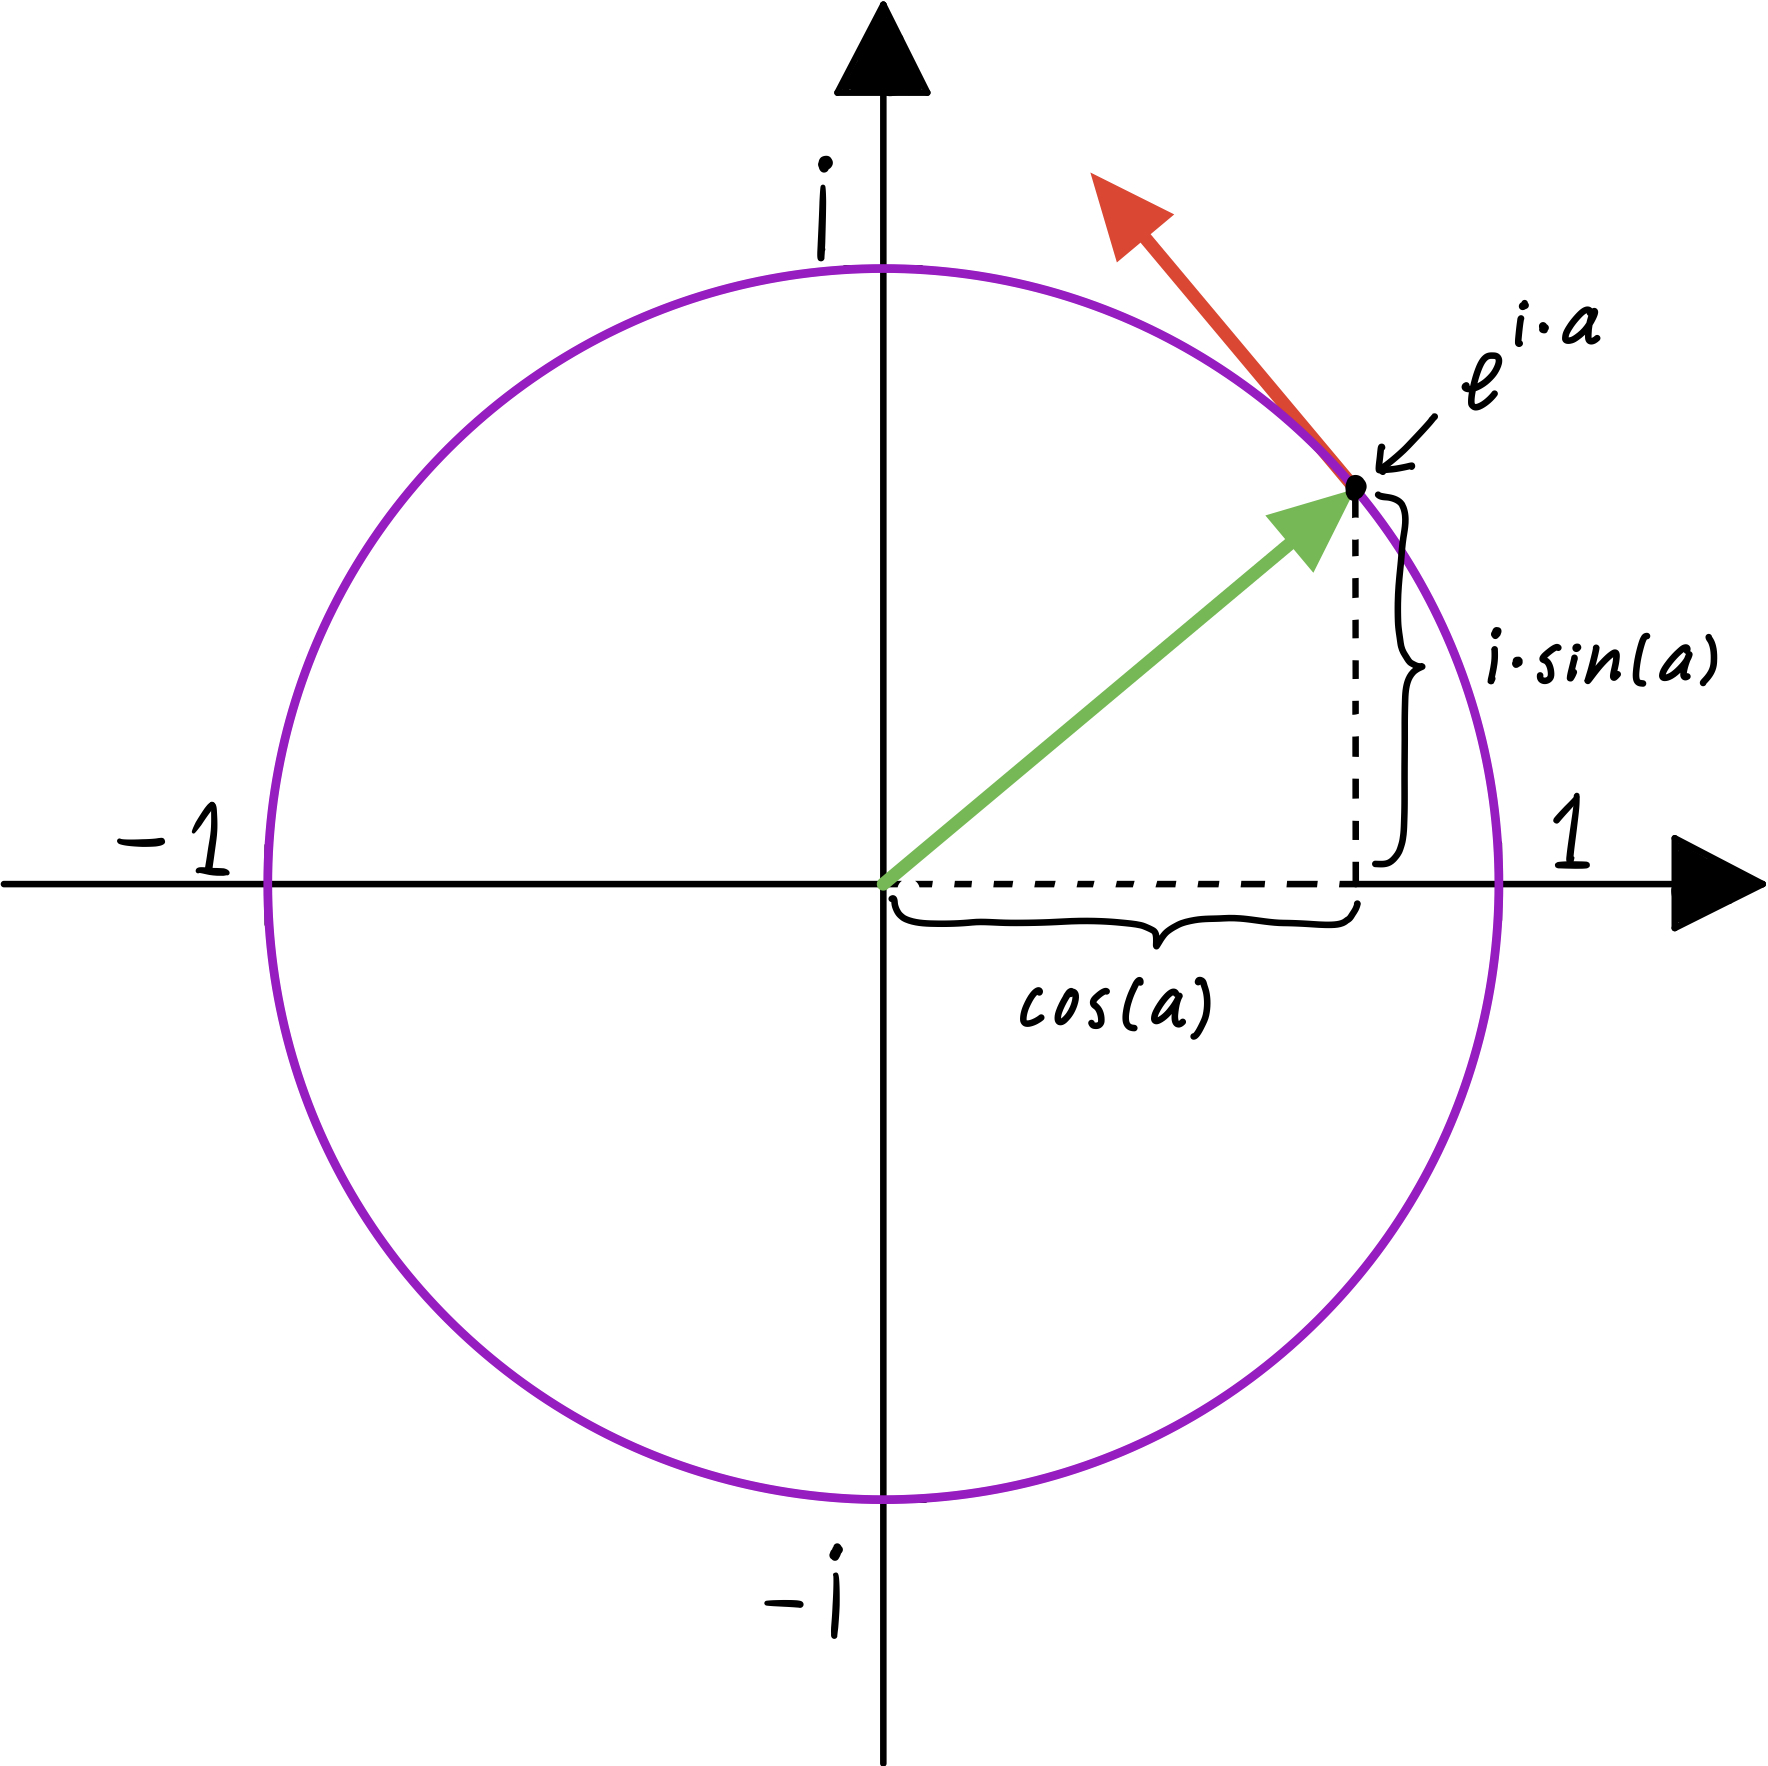
\includegraphics[width=50ex]{photos/chapter2/4.jpeg}
\end{figure}
\bigskip

Därmed är det rimligt att $ e^{ix} = \cos x + i\sin x $, vilket var målet att försöka visa.

% ------------------------------------------------------------------------------------------------------------------------------------------------------------------------
\newpage
\section{Simulering av himlakroppars rörelse}

Målet med detta kapitel är att beskriva matematiken bakom ett en generalisering av ett dynamiskt system som beskriver hur något antal himlakroppar rör sig relativt till ett koordinatsystem, 
när de påverkar varann med gravitation enligt newtons gravitationslag. För att sedan simulera ett valt dynamiskt system så behöver vi sedan veta alla himlakroppars koordinater i det valda koordinatsystemet och deras hastigheter och i vilken riktning de pekar, 
samt allas massor för det är vad som avgör med vilken kraft de drar på varann.
\bigskip

Vi börjar med att definiera en positionsvektorfunktion som beskriver positionen över tid för någon planet $ i $;
\bigskip

\bigskip
\hspace{5ex}
$ \vec{s_i} = 
    \begin{bmatrix}
    x_i \\
    y_i \\
    z_i 
    \end{bmatrix} $
\bigskip
\bigskip

$ x_i $, $ y_i $ och $ z_i $ är alla funktioner av tid men jag skriver inte ut dem som $ x_i(t) $ för det kommer att se kladdigt ut senare när uttrycken blir större. 
\bigskip

\bigskip
\hspace{5ex}
$ \dot \vec{s_i} = 
    \begin{bmatrix}
    \dot x_i \\
    \dot y_i \\
    \dot z_i 
    \end{bmatrix} = \diff{\vec{s}}{t} $

\bigskip
\hspace{5ex}
$ \ddot \vec{s_i} = 
    \begin{bmatrix}
    \ddot x_i \\
    \ddot y_i \\
    \ddot z_i 
    \end{bmatrix} $
\bigskip
\bigskip

Om vi deriverar $ \vec{s_i} $ så får vi fram hastighetsvektorfunktionen för planet $ i $, 
och om vi deriverar igen så får vi accelerationsvektorfunktionen för planet $ i $. 
För att göra det stilrenare så kan vi skriva derivatan av $ \vec{s_i} $ som $ \dot \vec{s_i} $ med en prick ovanför, 
så andraderivatan har då två prickar ovanför. Samma notation gäller även för $ x_i $, $ y_i $ och $ z_i $.
När vi väl skapar ett system så måste vi välja positionen för alla planeter och deras massor, 
men det som sedan styr hur systemet utvecklar sig är ju såklart gravitationen. 
Gravitationen är vad som styr accelerationen för planeten $ i $ vilket i sin tur förändrar hastigheten som i sin tur förändrar positionen, över tid. 
Om vi förstår gravitationen så följer resten.
\bigskip

Många är nog familjär med newtons gravitationslag, som ofta bara uttrycks i en dimension. Vi vill såklart ha den i tre.
\bigskip

\bigskip
\hspace{5ex}
$ F = G\dfrac{m_1m_2}{r^2} $ 
\bigskip
\bigskip

$ F $ är då kraften som verkar på båda planeterna i riktning mot varann, 
$ m_1 $ och $ m_2 $ är planeternas massor, 
$ r $ är avståndet mellan planeternas mittpunkter och $ G $ är gravitationskonstanten som beskriver hur stark gravitationen är. 
Det intressanta med vektorer är att vi kan dela upp dem i summor av skalärfunktioner multiplicerat med basvektorerna i koordinatsystemet, 
så som vi gjorde med positionsvektorfunktionen.
\bigskip

\bigskip
\hspace{5ex}
$ F_{ijx} = G\dfrac{m_im_j}{r^2} \cdot \dfrac{r_x}{r} = m_i \ddot x_{ij} $ 
\bigskip

\hspace{10ex}
$ \Updownarrow $
\bigskip

\hspace{5ex}
$ \ddot x_{ij} = G\dfrac{m_j}{r^2} \cdot \dfrac{r_x}{r} $
\bigskip

Med $ \ddot x_{ij} $ så menar jag accelerationen för planet $ i $ p.g.a planet $ j $ i $ x $-led. 
Om det hade stått $ \ddot x_{ji} $ så hade det varit accelerationen för planet $ j $ p.g.a planet $ i $ i $ x $-led.
Anledningen varför jag multiplicerar uttrycket med $ \dfrac{r_x}{r} $ är för att om avståndet mellan planeterna är $ r $ men vi vill ha accelerationen i $ x $-led så måste vi ta hänsyn till att accelerationen i x-led bara är en andel av den totala accelerationen,
och därmed multiplicerar vi med hur stort avståndet är i $ x $-led dividerat med det totala avståndet. En visualisering för vad jag menar:
\bigskip

\bigskip
\hspace{5ex}
$ r $ : lila pil
\bigskip

\hspace{5ex}
$ r_x $: röd pil

\hspace{5ex}
$ r_y $: grön pil

\hspace{5ex}
$ r_z $: blå pil

\begin{figure}[H]
    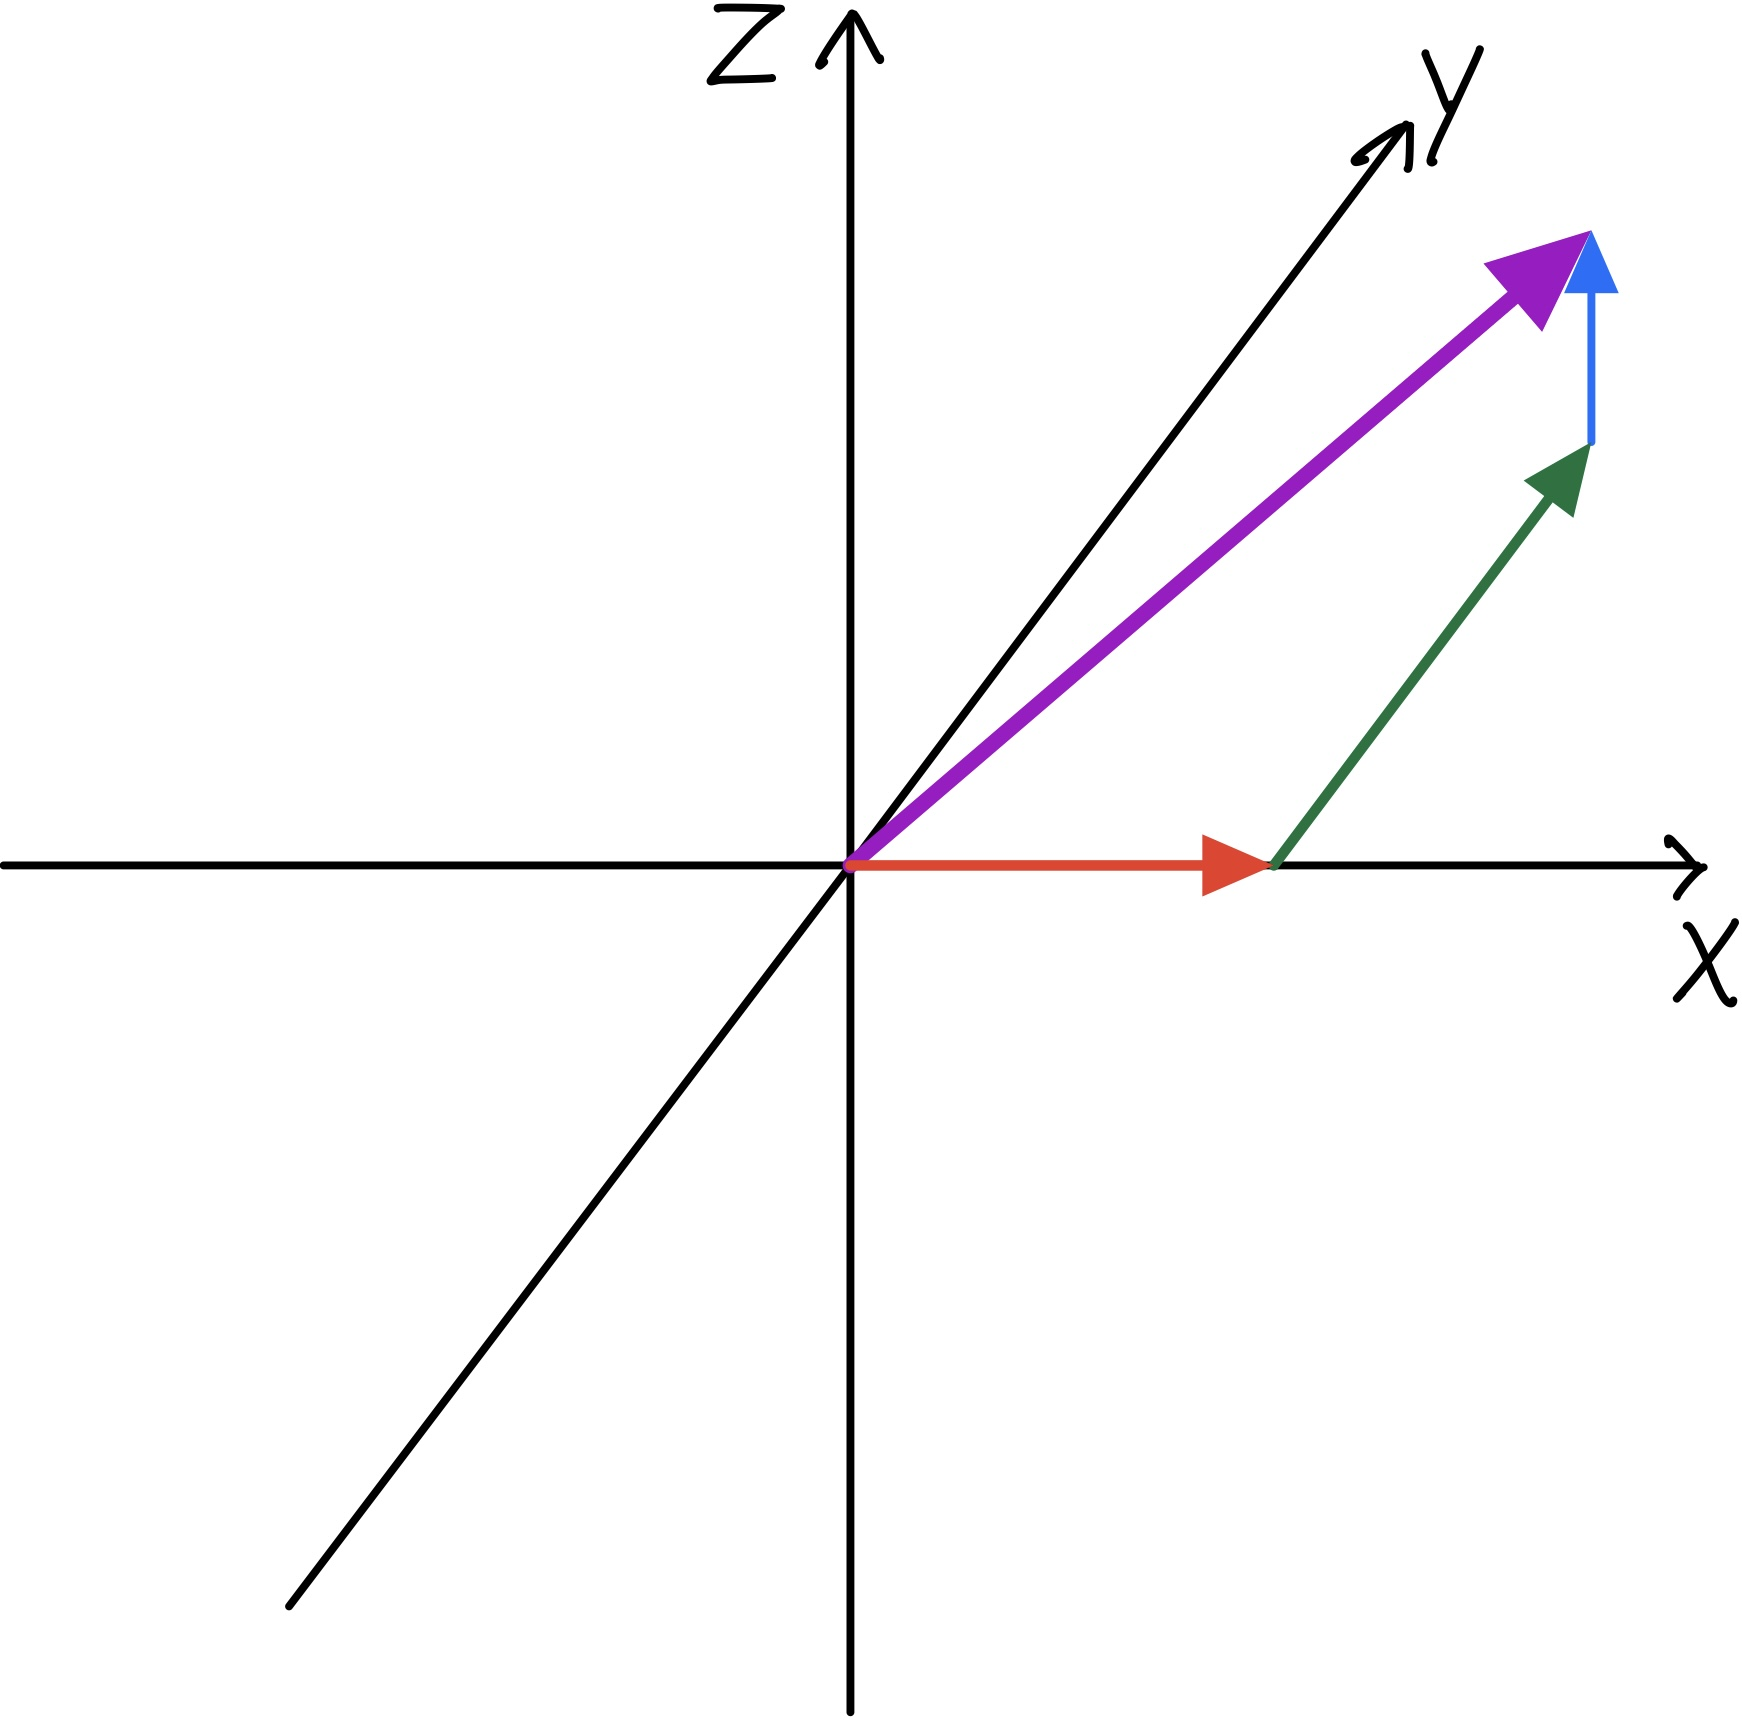
\includegraphics[width=50ex]{photos/chapter2/5.jpg}
    \centerline{planet $ i $ vid origo och planet $ j $ vid ändan av den lila pilen}
\end{figure}
\bigskip

storleken på $ r $ är alltså alltid positivt, men t.ex $ r_x $ kan vara negativ ifall planet $ j $ har en $ x $-koordinat som är mindre än för planet $ i $ och man mäter $ r_x $ ifrån perspektivet av planet $ i $;
\bigskip

\bigskip
\hspace{5ex}
$ r = \sqrt{(x_j - x_i)^2+(y_j - y_i)^2+(y_j - y_i)^2} $

\hspace{5ex}
$ r_x = x_j - x_i $
\bigskip

\bigskip
\hspace{5ex}
$ \ddot x_{ij} = G\dfrac{m_j}{r^2} \cdot \dfrac{r_x}{r} $
\bigskip

\hspace{10ex}
$ \Downarrow $
\bigskip

\hspace{5ex}
$ \ddot x_{ij} = G\dfrac{m_j}{(\sqrt{(x_j - x_i)^2+(y_j - y_i)^2+(y_j - y_i)^2})^2} \cdot \dfrac{x_j - x_i}{\sqrt{(x_j - x_i)^2+(y_j - y_i)^2+(y_j - y_i)^2}} $
\bigskip

\hspace{10ex}
$ \Updownarrow $
\bigskip

\hspace{5ex}
$ \ddot x_{ij} = \dfrac{Gm_j(x_j - x_i)}{((x_j - x_i)^2+(y_j - y_i)^2+(y_j - y_i)^2)^{3/2}} $
\bigskip
\bigskip

Samma argument kan vi använda för $ y $ och $ z $ också, så vi kan skriva hela accelerationen som för planet $ i $ p.g.a $ j $ som;
\bigskip

\bigskip
\hspace{5ex}
$ \ddot \vec{s_{ij}} = 
    \begin{bmatrix}
    \ddot x_{ij} \\
    \ddot y_{ij} \\
    \ddot z_{ij} 
    \end{bmatrix} $
\bigskip

\hspace{10ex}
$ \Updownarrow $
\bigskip

\hspace{5ex}
$ \ddot \vec{s_{ij}} = 
    \begin{bmatrix}
    \dfrac{Gm_j(x_j - x_i)}{((x_j - x_i)^2+(y_j - y_i)^2+(y_j - y_i)^2)^{3/2}} \\ \\
    \dfrac{Gm_j(y_j - y_i)}{((x_j - x_i)^2+(y_j - y_i)^2+(y_j - y_i)^2)^{3/2}} \\ \\
    \dfrac{Gm_j(z_j - z_i)}{((x_j - x_i)^2+(y_j - y_i)^2+(y_j - y_i)^2)^{3/2}}
    \end{bmatrix} $
\bigskip
\bigskip

Vad händer om vi har fler än två planeter i systemet? Alla planeter drar på varann med någon kraft, 
så accelerationen för planet $ i $ beror då på alla resterande planeter i systemet. 
Ifall vi har ett system med $ n $ planeter, och planet $ i $ är en av dem, 
$ i \in \left(1, n\right) $,
så kan vi summera ihop den påverkan som alla resterande planeter i systemet har på planet $ i $ såhär;
\bigskip

\bigskip
$ \ddot \vec{s_{i}} =
    \begin{cases}
        \begin{bmatrix}
            \sum\limits_{j=i + 1}^{n} \dfrac{Gm_j(x_j - x_i)}{((x_j - x_i)^2+(y_j - y_i)^2+(y_j - y_i)^2)^{3/2}} \\ \\
            \sum\limits_{j=i + 1}^{n} \dfrac{Gm_j(y_j - y_i)}{((x_j - x_i)^2+(y_j - y_i)^2+(y_j - y_i)^2)^{3/2}} \\ \\
            \sum\limits_{j=i + 1}^{n} \dfrac{Gm_j(z_j - z_i)}{((x_j - x_i)^2+(y_j - y_i)^2+(y_j - y_i)^2)^{3/2}}
            \end{bmatrix} & \text{, } i = 1 \\ \\
        \begin{bmatrix}
            \sum\limits_{j=1}^{i - 1} \dfrac{Gm_j(x_j - x_i)}{((x_j - x_i)^2+(y_j - y_i)^2+(y_j - y_i)^2)^{3/2}} + \sum\limits_{j=i + 1}^{n} \dfrac{Gm_j(x_j - x_i)}{((x_j - x_i)^2+(y_j - y_i)^2+(y_j - y_i)^2)^{3/2}} \\ \\
            \sum\limits_{j=1}^{i - 1} \dfrac{Gm_j(y_j - y_i)}{((x_j - x_i)^2+(y_j - y_i)^2+(y_j - y_i)^2)^{3/2}} + \sum\limits_{j=i + 1}^{n} \dfrac{Gm_j(y_j - y_i)}{((x_j - x_i)^2+(y_j - y_i)^2+(y_j - y_i)^2)^{3/2}} \\ \\
            \sum\limits_{j=1}^{i - 1} \dfrac{Gm_j(z_j - z_i)}{((x_j - x_i)^2+(y_j - y_i)^2+(y_j - y_i)^2)^{3/2}} + \sum\limits_{j=i + 1}^{n} \dfrac{Gm_j(z_j - z_i)}{((x_j - x_i)^2+(y_j - y_i)^2+(y_j - y_i)^2)^{3/2}}
            \end{bmatrix} & \text{, } i \in \left[2, (n - 1)\right] \\ \\
        \begin{bmatrix}
            \sum\limits_{j=1}^{i - 1} \dfrac{Gm_j(x_j - x_i)}{((x_j - x_i)^2+(y_j - y_i)^2+(y_j - y_i)^2)^{3/2}} \\ \\
            \sum\limits_{j=1}^{i - 1} \dfrac{Gm_j(y_j - y_i)}{((x_j - x_i)^2+(y_j - y_i)^2+(y_j - y_i)^2)^{3/2}} \\ \\
            \sum\limits_{j=1}^{i - 1} \dfrac{Gm_j(z_j - z_i)}{((x_j - x_i)^2+(y_j - y_i)^2+(y_j - y_i)^2)^{3/2}}
            \end{bmatrix} & \text{, } i = n
    \end{cases} $
\bigskip
\bigskip

Det blev ett väldigt stort uttryck men vi kan bryta ner det och förstå vad som står här. 
Som det står i uttrycket så gäller den övre parten om $ i = 1 $. 
Om vi tittar på accelerationen i $ x $-led, alltså detta uttryck högst up:
\bigskip

\bigskip
\hspace{5ex}
$ \sum\limits_{j=i + 1}^{n} \dfrac{Gm_j(x_j - x_i)}{((x_j - x_i)^2+(y_j - y_i)^2+(y_j - y_i)^2)^{3/2}} $
\bigskip
\bigskip

Då så ser vi att summeringen först adderar accelerationen för planet $ i $ som konsekvens av planet $ i + 1 $, 
vilket alltså är planet $ 2 $ i detta fall.
Efter det så adderar den också accelerationen för planet $ i $ som konsekvens av planet $ i + 2 $,
vilket är planet $ 3 $.
Såhär fortsätter det upp till planet $ n $ som är den sista planeten i systemet. 
Summeringen lägger alltså ihop den totala accelerationen som planet $ i $ får i $ x $-led som konsekvens av alla andra planeter i systemet.
Under den summeringen så finns samma uttryck men utbytt med $ y $ och sedan $ z $ för att göra samma sak i $ y $-led och $ z $-led.
\bigskip

Nästa möjliga fall är då $ i \in \left[2, n - 1\right] $, vilket betyder att planet $ i $ kan vara planet 2 eller uppåt förutom att vara planet $ n $.
I detta fall så måste vi först addera ihop den totala accelerationen som konsekvens av planeterna med lägre nummer än planet $ i $, 
vilket ser ut såhär för $ x $-ledet:
\bigskip

\bigskip
\hspace{5ex}
$ \sum\limits_{j=1}^{i - 1} \dfrac{Gm_j(x_j - x_i)}{((x_j - x_i)^2+(y_j - y_i)^2+(y_j - y_i)^2)^{3/2}} $
\bigskip
\bigskip

Summeringen börjar med att addera accelerationen för planet $ i $ som konsekvens av planet $ 1 $, 
och sedan samma sak med planet $ 2 $, o.s.v. fram tills planet $ i - 1 $.
Vi kan ju inte addera accelerationen för planet $ i $ som konsekvens av planet $ i $ för det skulle resultera i att vi måste dividera med $ 0 $ då avståndet mellan samma planet är $ 0 $,
så vi får istället skapa en till summa som ser likadan ut förutom att den börjar vid planet $ i + 1 $ och slutar vid planet $ n $. 
Detta kan ses i uttrycket för accelerationen i $ x $-led när kravet $ i \in \left[2, n - 1\right] $ är uppfyllt:
\bigskip

\bigskip
\hspace{5ex}
$ \sum\limits_{j=1}^{i - 1} \dfrac{Gm_j(x_j - x_i)}{((x_j - x_i)^2+(y_j - y_i)^2+(y_j - y_i)^2)^{3/2}} + \sum\limits_{j=i + 1}^{n} \dfrac{Gm_j(x_j - x_i)}{((x_j - x_i)^2+(y_j - y_i)^2+(y_j - y_i)^2)^{3/2}} $
\bigskip
\bigskip

Samma argument används för accelerationen i $ y $-led och $ z $-led.
\bigskip

När $ i = n $ så görs en likadan summering förutom att vi startar med att addera accelerationen som konsekvens av planet $ 1 $ och sedan alla resterande planeter upp till planet $ i - 1 $ för planet $ i $ är ju som sagt planet $ n $.
Såhär ser det ut i $ x $-led:
\bigskip

\bigskip
\hspace{5ex}
$ \sum\limits_{j=1}^{i - 1} \dfrac{Gm_j(x_j - x_i)}{((x_j - x_i)^2+(y_j - y_i)^2+(y_j - y_i)^2)^{3/2}} $
\vspace{24pt plus 4pt minus 4pt}
spc

Samma argument används såklart också för accelerationen i $ y $-led och $ z $-led.
\bigskip

Allt detta sammanlagt brukar vanligtvis skrivas på ett annat vis där man skriver ut vektorer istället för alla dess komponenter, och det är lite mer kompakt:
\bigskip

\bigskip
\hspace{5ex}
$ \ddot \vec{s_{i}} = \sum\limits_{j \neq i}^{} \dfrac{Gm_j}{r_{ij}^3}\vec r_{ij} $
\vspace{24pt plus 4pt minus 4pt}

Jag föredrar dock när det är helt utskrivet som på sida 18 för jag tycker det är tydligare.
Hur använder vi då detta för att skapa ett dynamiskt system?
Vi börjar med att definiera en vektorfunktion av tid som innehåller positionen och hastigheten för alla planeter i systemet och sedan deriverar vi den:
\bigskip

\bigskip
\hspace{5ex}
$ \vec{u}(t) = 
    \begin{bmatrix}
        \vec s_1 \\
        \dot \vec s_1 \\
        \vec s_2 \\
        \dot \vec s_2 \\
        \vdots \\
        \vec s_n \\
        \dot \vec s_n \\
    \end{bmatrix}
$ 
$ \text{ } $
$ \text{ } $
$ \Leftrightarrow $
$ \text{ } $
$ \text{ } $
$ \dot \vec{u}(t) = 
    \begin{bmatrix}
        \dot \vec s_1 \\
        \ddot \vec s_1 \\
        \dot \vec s_2 \\
        \ddot \vec s_2 \\
        \vdots \\
        \dot \vec s_n \\
        \ddot \vec s_n \\
    \end{bmatrix}
$ 
\vspace{24pt plus 4pt minus 4pt}

Om vi nu ska använda detta för att se hur systemet utvecklar sig så måste vi först välja något antal planeter, $ n $, 
sedan måste vi ge dem någon startposition i vårt koordinatsystem och sedan måste de också få någon starthastighet i någon riktning.
Detta görs genom att välja startvärdena vid $ t = 0 $ för alla positionsvektorfunktioner och hastighetsvektorfunktioner för alla planeter, 
som finns i vektorfunktionen $ \vec u(t) $.
När vi har gett planeterna varsin position och hastighet med riktning vid $ t = 0 $ så kan vi intressera oss av hur hastigheterna och därmed positionerna kommer att förändras över tid,
vilket vi kan få reda på genom accelerationen som är en konsekvens av gravitationskrafterna mellan alla planeter.
För det behöver vi också ange massan hos varje planet i systemet.
Vi har redan beskrivit accelerationen för någon planet $ i $ i ett system med $ n $ planeter, 
så vi kan nu ge värden på alla komponenter i $ \vec u(t) $ och $ \dot \vec u(t) $ vid $ t = 0 $.
För att hoppa fram i värden på $ t $ förbi $ t = 0 $ till tiden $ t = t_a $ så kan vi använda eulers stegmetod:
\vspace{24pt plus 4pt minus 4pt}

\hspace{5ex}
$ \dot \vec u(t) = f(t, \vec u(t)) $
\bigskip

\hspace{5ex}
$ \vec u_0 = \vec u(t_0) $
\bigskip

\hspace{5ex}
$ \vec u_{k+1} = \vec u_k + hf(t_k, \vec u_k) $
\bigskip

\hspace{5ex}
$ \vec u_k \approx \vec u(t_k) $
\vspace{24pt plus 4pt minus 4pt}

Vi kan därmed veta systemets information (alla planeters position och hastighet med riktning) fram i tiden med hjälp av att ta små diskreta tidssteg och se hur systemet utvecklar sig. 
Om en planet rör sig med en hastighet åt något håll så kan vi veta hur positionen förflyttar sig om vi multiplicerar med ett litet tidssteg, 
och sedan vet vi hur hastigheten förändras över samma tid genom att multiplicera accelerationen med ett litet tidssteg. 
På det sättet hoppar vi alltså fram, enligt eulers stegmetod. 
Det finns många andra mer avancerade stegmetoder för numeriska lösningar till differentialekvationer,
men eulers stegmetod är den enklaste och den fungerar ifall precisionen inte är så viktig.

% ------------------------------------------------------------------------------------------------------------------------------------------------------------------------
\newpage
\section{Mandelbrottmängden}
\begin{figure}[H]
    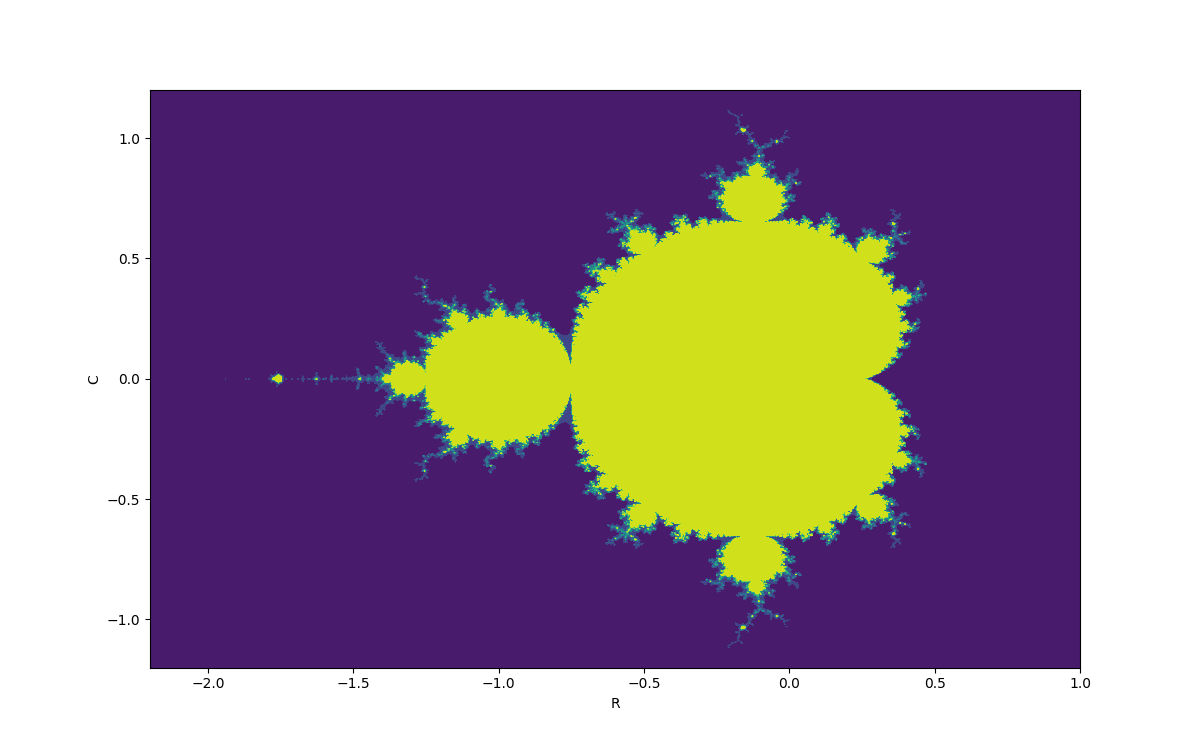
\includegraphics[width=\linewidth]{photos/chapter4/1.png}
    \centerline{(renderad med python och matplotlib)}
\end{figure}
\bigskip

Detta är en avbild av ett mönster som snabbt hittas om man googlar på "Mandelbrot Set".
Vad är då det? \bigskip 

\textbf{Mandelbrottmängden}, så som det heter på svenska, 
är den mängden punkter $ c $ i det komplexa talplanet där denna rekursiva talföljd konvergerar när $ n $ går emot oändligheten.

\begin{align*}
    z_0 &= 0\\
    z_{n+1} &= z_n^2 + c
\end{align*} \bigskip

De punkter som syns som gula i bilden är inom denna mängd, 
och där det övergår mot lila så visar färggradienten ungefär hur snabbt talföljden divergerar. \bigskip 

ÄR INTE FÄRDIG HÄR

% ------------------------------------------------------------------------------------------------------------------------------------------------------------------------
\newpage
\section{Dubbelpendeln} 

I detta kapitel så är målet att beskriva rörelsen för en dubbelpendel genom att komma fram med ekvationerna för vinkelaccelerationen för vardera pendel, 
då det gör det möjligt att sedan använda en numerisk metod för att simulera dubbelpendeln. Vi börjar med att definiera vad vi menar med dubbelpendeln: \bigskip 

\begin{figure}[H]
    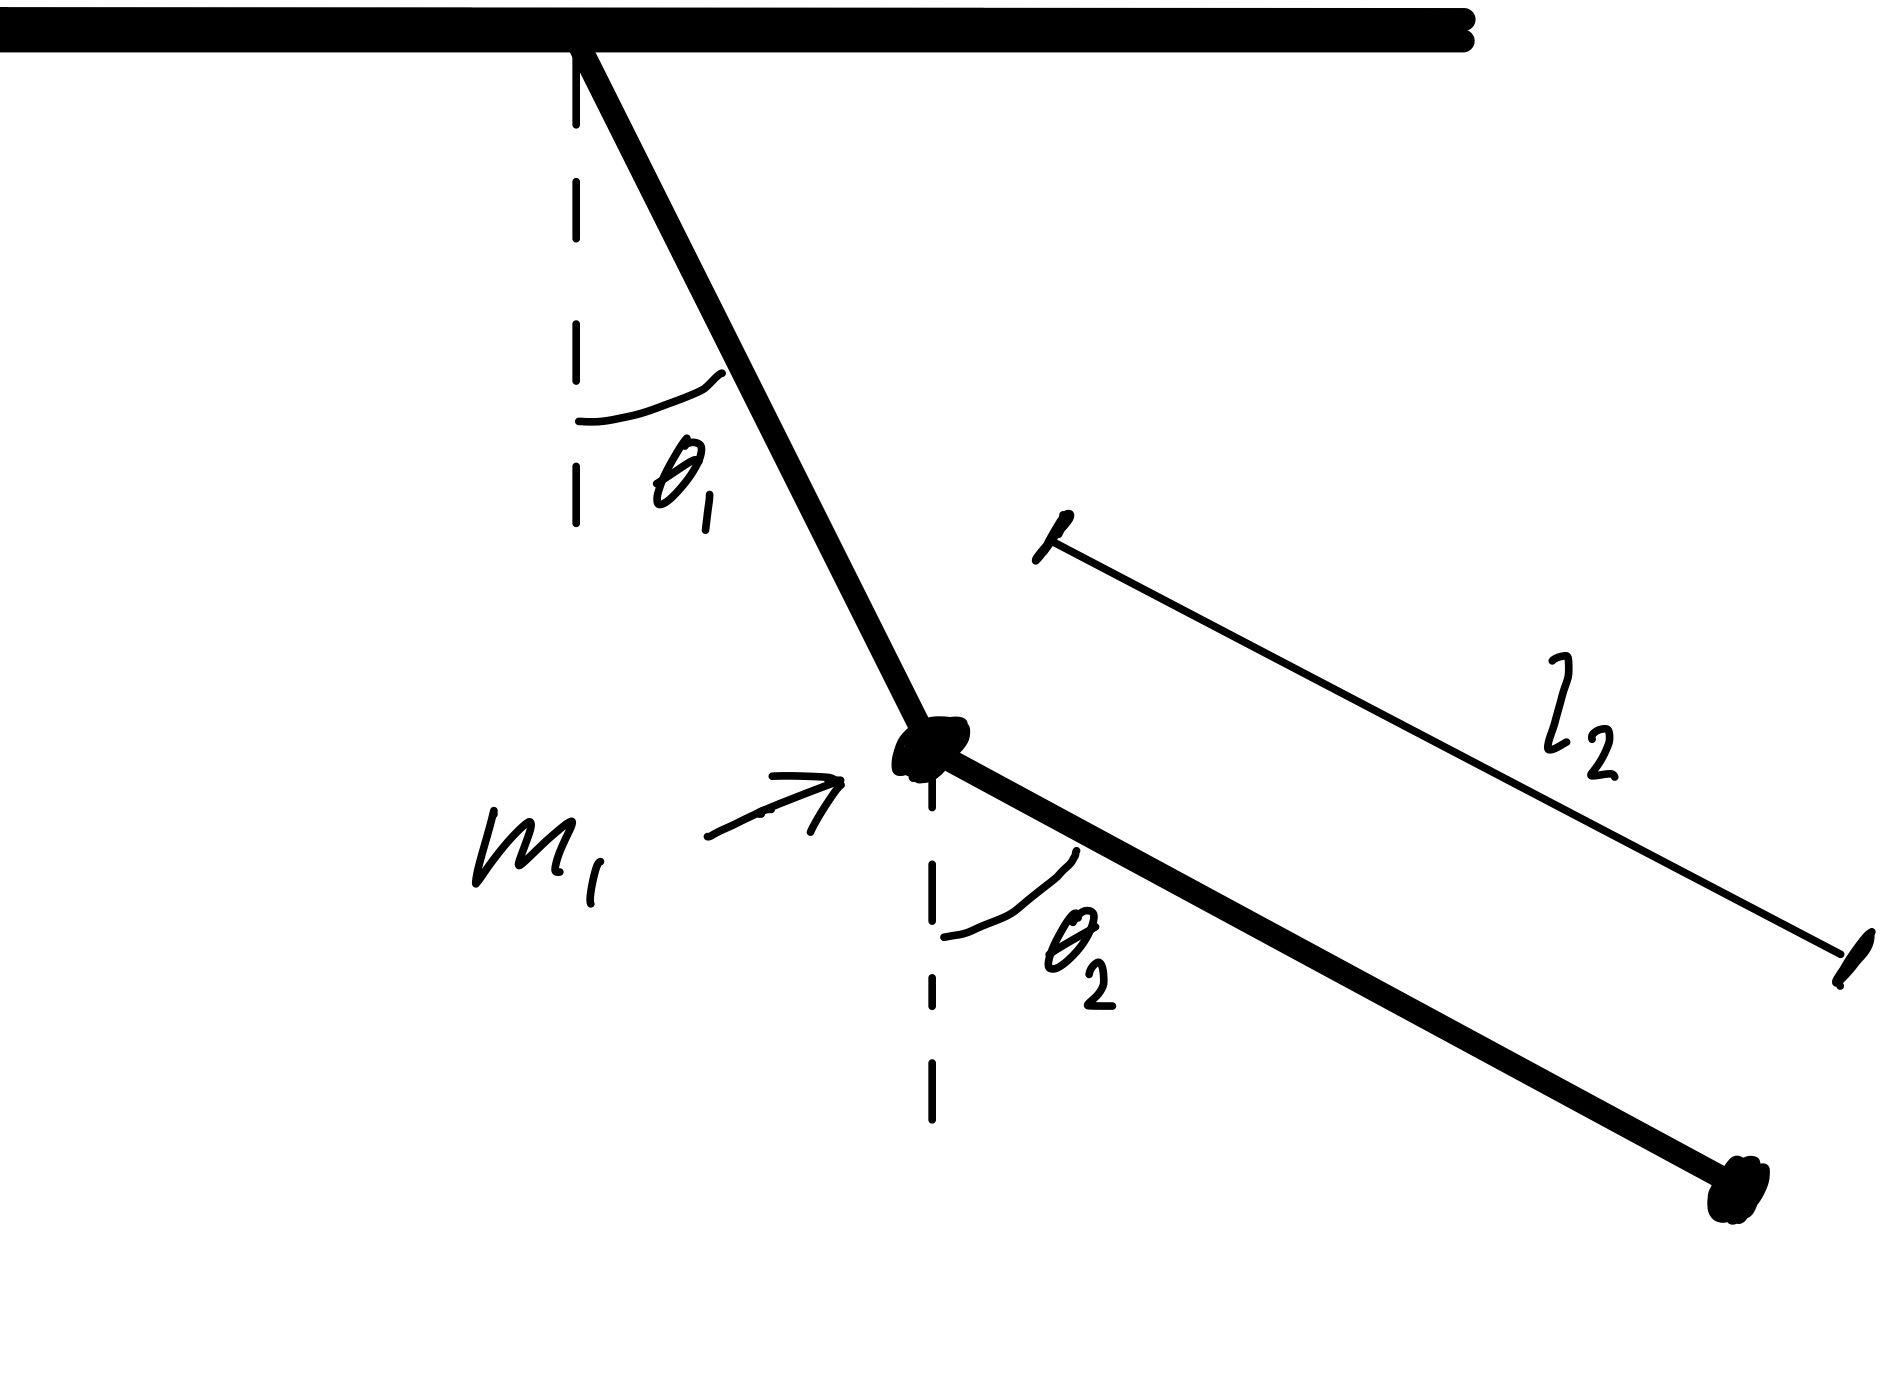
\includegraphics[width=50ex]{photos/chapter5/1.jpg}
\end{figure} \bigskip 

Pendel 1 har sitt fäste i origo i ett koordinatsystem av $ \mathbb{R}^2 $. 
$ y $-axeln är positiv över origo och är vertikal i denna bild, 
och $ x $-axeln är positiv till höger om origo och är horisontell i denna bild. 
Pendel 1 har alltså en vinkel $ \theta_1 $ som är $ 0 $ radianer när pendel 1 ligger rakt ner längs gravitationsfältet. 
Pendel 1 har också en längd $ L_1 $ och en partikel längst ut med massan $ m_1 $. Samma gäller då för pendel 2. 
Utifrån detta så kan vi lätt beskriva positionen, hastigheten och accelerationen för de två partiklarna: \bigskip 

\begin{align}
    x_1 &= L_1\sin\theta_1 \\
    \dot x_1 &= \dot \theta_1L_1\cos \theta_1 \\
    \ddot x_1 &= \ddot \theta_1L_1\cos \theta_1 - \dot \theta_1^2L_1\sin \theta_1 \\
    y_1 &= -L_1\cos\theta_1 \\
    \dot y_1 &= \dot \theta_1L_1\sin \theta_1 \\
    \ddot y_1 &= \ddot \theta_1L_1\sin \theta_1 + \dot \theta_1^2L_1\cos \theta_1
\end{align}

\begin{align}
    x_2 &= x_1 + L_2\sin\theta_2 \\
    \dot x_2 &= \dot x_1 + \dot \theta_2L_2\cos \theta_2 \\
    \ddot x_2 &= \ddot x_1 + \ddot \theta_2L_2\cos \theta_2 - \dot \theta_2^2L_2\sin \theta_2 \\
    y_2 &= y_1 -L_2\cos\theta_2 \\
    \dot y_2 &= \dot y_1 + \dot \theta_2L_2\sin \theta_2 \\
    \ddot y_2 &= \ddot y_1 + \ddot \theta_2L_2\sin \theta_2 + \dot \theta_2^2L_2\cos \theta_2
\end{align} \bigskip 

Enbart detta hjälper dock inte så värst mycket. 
Vi behöver veta vinkelaccelerationerna, 
vinkelhastigheterna och vinklarna för att kunna veta vad de motsvarar i $ x $ och $ y $.
För att kunna ta reda på dem så tänker jag använda mig av Lagrangemekanik.

\subsubsection*{\textbf{Lagrangemekanik}}
\hspace{5ex} 

Till skillnad från newtonsk mekanik så behöver vi inte analysera några krafter, 
men istället så använder vi oss av restriktionerna för skalären energi i systemet genom konceptet som kallas \textit{The Principle of Least Action}.
\textit{The Principle of Least Action} säger att den så kallade \textit{Action} är definierad som: \bigskip 

\begin{align}
    S = \int_{t_2}^{t_1} L(q^{i}, \dot q^{i}, t)dt
\end{align} \bigskip 

där $ q^{i} $ och $ \dot q^{i} $ är generaliserade koordinater och hastigheter med riktning, 
och $ L $ är \textit{lagrangen} av systemet som definieras som: \bigskip 

\begin{align}
    L = T - U
\end{align} \bigskip 

där $ T $ är den totala rörelseenergin i systemet och $ U $ är den totala potentiella energin i systemet. 
Om den så kallade \textit{Action} är vid sin extrempunkt, som då visar den väg som systemet faktiskt tar, så stämmer denna ekvation som kallas \textit{Euler-Lagrange equation}: \bigskip 

\begin{align}
    \dfrac{d}{dt}\dfrac{\partial L}{\partial \dot q^{i}} - \dfrac{\partial L}{\partial q^{i}} = 0
\end{align} \bigskip 

\subsubsection*{\textbf{Uträkning}}
\hspace{5ex} 

Det första vi alltså behöver göra är att ta fram \textit{lagrangen} i systemet, 
som vi kan få fram om vi vet rörelseenergin och den potentiella energin i systemet enligt ekvation (14). \bigskip 

\begin{align}
    T &= \dfrac{1}{2}\sum_{i=1}^{n} m_iv_i^2 = \\
      &= \dfrac{1}{2}\sum_{i=1}^{n} m_i(\dot x_i^2 + \dot y_i^2) = \\
      &= \dfrac{1}{2}\sum_{i=1}^{n} m_i((\sum_{j=1}^{i}\dot \theta_jL_j\cos \theta_j)^2 + (\sum_{j=1}^{i}\dot \theta_jL_j\sin \theta_j)^2) = \\
      &= \dfrac{1}{2}\sum_{i=1}^{n} m_i((\sum_{j=1}^{i} \dot\theta_j^2L_j^2\cos^2\theta_j + 2\sum_{j \neq k}^{i} \dot\theta_jL_j\cos\theta_j\dot\theta_kL_k\cos\theta_k) + (\sum_{j=1}^{i} \dot\theta_j^2L_j^2\sin^2\theta_j + 2\sum_{j \neq k}^{i} \dot\theta_jL_j\sin\theta_j\dot\theta_kL_k\sin\theta_k)) = \\
      &= \dfrac{1}{2}\sum_{i=1}^{n} m_i((\sum_{j=1}^{i} \dot\theta_j^2L_j^2 + 2\sum_{j \neq k}^{i} \dot\theta_j\dot\theta_kL_jL_k\cos(\theta_j - \theta_k)) = \\
      &= \sum_{i=1}^{n} (\sum_{j=1}^{i} \dfrac{1}{2}m_i\dot\theta_j^2L_j^2 + \sum_{j \neq k}^{i} m_i\dot\theta_j\dot\theta_kL_jL_k\cos(\theta_j - \theta_k))
\end{align} \bigskip 

Nu har vi ett generellt uttryck för rörelseenergin i pendeln, 
och tro mig, 
det är kortare att skriva det som summor. 
Nu ska vi göra samma sak med den potentiella energin: \bigskip 

\begin{align}
    U &= \sum_{i=1}^{n} m_igy_i = \\
      &= \sum_{i=1}^{n} m_ig(\sum_{j=1}^{i} -L_j\cos\theta_j) = \\
      &= -\sum_{i=1}^{n}\sum_{j=1}^{i} m_igL_j\cos\theta_j =
\end{align} \bigskip 

Lagrangen $ L $ är alltså:

\begin{align}
    L &= T - U \\
      &= \sum_{i=1}^{n} (\sum_{j=1}^{i} \dfrac{1}{2}m_i\dot\theta_j^2L_j^2 + \sum_{j \neq k}^{i} m_i\dot\theta_j\dot\theta_kL_jL_k\cos(\theta_j - \theta_k)) + \sum_{i=1}^{n}\sum_{j=1}^{i} m_igL_j\cos\theta_j = \\
      &= \sum_{i=1}^{n} (\sum_{j=1}^{i} \dfrac{1}{2}m_i\dot\theta_j^2L_j^2 + \sum_{j \neq k}^{i} m_i\dot\theta_j\dot\theta_kL_jL_k\cos(\theta_j - \theta_k) + \sum_{j=1}^{i} m_igL_i\cos\theta_i)
\end{align} \bigskip 

Nu kan man ju undra varför jag inte gjorde en n-pendel utifrån detta. 
Det har att göra med att jag inte har någon aning hur jag sedan ska kunna derivera detta på några sätt som vi kommer att behöva göra. 
Jag har kunnat hitta lösningen på dem men jag förstår inte hur man kom fram med det, så jag skriver bara det jag förstår här. 
Om du vill kika på n-pendeln så fortsätt här istället (den har dock valt 1 kg och 1 meter för alla pendlar, pga förenklade beräkningar): https://travisdoesmath.github.io/pendulum-explainer/ \bigskip 

Om vi väljer att $ n = 2 $ för den generella lagrangen för n-pendeln så kan vi få fram lagrangen för dubbelpendeln: \bigskip 

\begin{align}
    L &= \sum_{i=1}^{2} (\sum_{j=1}^{i} \dfrac{1}{2}m_i\dot\theta_j^2L_j^2 + \sum_{j \neq k}^{i} m_i\dot\theta_j\dot\theta_kL_jL_k\cos(\theta_j - \theta_k) + \sum_{j=1}^{i} m_igL_i\cos\theta_i) = \\
    &= (\dfrac{1}{2}m_1\dot\theta_1^2L_1^2 + m_1gL_1\cos\theta_1) + (\dfrac{1}{2}m_2\dot\theta_1^2L_1^2 + \dfrac{1}{2}m_2\dot\theta_2^2L_2^2 + m_2\dot\theta_1\dot\theta_2L_1L_2\cos(\theta_1 - \theta_2) + m_2gL_1\cos\theta_1 + m_2gL_2\cos\theta_2) = \\
    &= \dfrac{1}{2}(m_1+m_2)\dot\theta_1^2L_1^2 + \dfrac{1}{2}m_2\dot\theta_2^2L_2^2 + \dfrac{1}{2}m_2\dot\theta_2^2L_2^2 + m_2\dot\theta_1\dot\theta_2L_1L_2\cos(\theta_1 - \theta_2) + (m_1+m_2)gL_1\cos\theta_1 + m_2L_2g\cos\theta_2
\end{align} \bigskip 

Om integralen av denna lagrange mellan två tidpunkter, 
som kallas action och ses i ekvation (13), 
värderas vid sin extrempunkt så stämmer ekvationen (15). 
Detta betyder att vi behöver derivera lagrangen över vinklarna, 
vinkelhastigheterna och tidsderivatan av vinkelhastighetsderivatorna av lagrangen: \bigskip 

\begin{align}
    \dfrac{\partial L}{\partial\theta_1} &= -L_1g(m_1+m_2)\sin\theta_1 - m_2\dot\theta_1\dot\theta_2L_1L_2\sin(\theta_1 - \theta_2)
\end{align}
\begin{align}
    \dfrac{\partial L}{\partial\dot\theta_1} &= (m_1 + m_2)\dot\theta_1L_1^2 + m_2\dot\theta_2L_1L_2\cos(\theta_1 - \theta_2) \\
    \dfrac{d}{dt} (\dfrac{\partial L}{\partial\dot\theta_1}) &= (m_1 + m_2)\ddot\theta_1L_1^2 + m_2\ddot\theta_2L_1L_2\cos(\theta_1 - \theta_2) - m_2\dot\theta_2L_1L_2\sin(\theta_1 - \theta_2)(\dot\theta_1 - \dot\theta_2)
\end{align} \bigskip 

Nu har vi de nödvändiga derivatorna för $ \theta_1 $, så vi använder dem för att senare kunna bryta ut vinkelaccelerationen: \bigskip 


\begin{align}
    \dfrac{d}{dt} (\dfrac{\partial L}{\partial\dot\theta_1}) - \dfrac{\partial L}{\partial\theta_1} &= 0
\end{align}
\begin{multline}
    (m_1 + m_2)\ddot\theta_1L_1^2 + m_2\ddot\theta_2L_1L_2\cos(\theta_1 - \theta_2) - m_2\dot\theta_2L_1L_2\sin(\theta_1 - \theta_2)(\dot\theta_1 - \dot\theta_2) + L_1g(m_1+m_2)\sin\theta_1 \\ - m_2\dot\theta_1\dot\theta_2L_1L_2\sin(\theta_1 - \theta_2) = 0
\end{multline}
\begin{align}
    \ddot\theta_1 &= \dfrac{-m_2\ddot\theta_2\cos(\theta_1 - \theta_2) - m_2\dot\theta_2^2L_2\sin(\theta_1 - \theta_2) - (m_1 + m_2)g\sin\theta_1}{(m_1 + m_2)L_1}
\end{align} \bigskip 

Nu gör vi exakt samma sak för $ \theta_2 $, hela alltet.

\begin{align}
    \dfrac{\partial L}{\partial\theta_2} &= m_2\dot\theta_1\dot\theta_2L_1L_2\sin(\theta_1 - \theta_2) - m_2L_2g\sin\theta_2
\end{align}
\begin{align}
    \dfrac{\partial L}{\partial\dot\theta_2} &= m_2\dot\theta_2L_2^2 + m_2\dot\theta_1L_1L_2\cos(\theta_1 - \theta_2) \\
    \dfrac{d}{dt} (\dfrac{\partial L}{\partial\dot\theta_2}) &= m_2\ddot\theta_2L_2^2 + m_2\ddot\theta_1L_1L_2\cos(\theta_1 - \theta_2) - m_2\dot\theta_1L_1L_2\sin(\theta_1 - \theta_2)(\dot\theta_1 - \dot\theta_2)
\end{align} \bigskip 

Nu har vi de nödvändiga derivatorna för $ \theta_2 $, så vi använder dem för att senare kunna bryta ut vinkelaccelerationen: \bigskip 
zw
\begin{align}
    \dfrac{d}{dt} (\dfrac{\partial L}{\partial\dot\theta_2}) - \dfrac{\partial L}{\partial\theta_2} &= 0
\end{align}
\begin{align}
    \ddot\theta_2L_2 + \ddot\theta_1L_1\cos(\theta_1 - \theta_2) - \dot\theta_1^2L_1\sin(\theta_1 - \theta_2) + g\sin\theta_2
\end{align}
\begin{align}
    \ddot\theta_2 &= \dfrac{-m_2\ddot\theta_2\cos(\theta_1 - \theta_2) - m_2\dot\theta_2^2L_2\sin(\theta_1 - \theta_2) - (m_1 + m_2)g\sin\theta_1}{(m_1 + m_2)L_1}
\end{align} \bigskip

Vi har nu båda dessa ekvationer som innehåller varann, så vi kan använda båda i kombination för att totalt lösa ut vardera vinkelacceleration: \bigskip 

\begin{align}
    \ddot\theta_1 &= \dfrac{-m_2\ddot\theta_2\cos(\theta_1 - \theta_2) - m_2\dot\theta_2^2L_2\sin(\theta_1 - \theta_2) - (m_1 + m_2)g\sin\theta_1}{(m_1 + m_2)L_1} \\
    \ddot\theta_2 &= \dfrac{-m_2\ddot\theta_2\cos(\theta_1 - \theta_2) - m_2\dot\theta_2^2L_2\sin(\theta_1 - \theta_2) - (m_1 + m_2)g\sin\theta_1}{(m_1 + m_2)L_1}
\end{align} \bigskip 

Först sätter vi in $ \ddot\theta_2 $ i högerledet av $ \ddot\theta_1 $ som genom en lång förenkling ger den första ekvationen här under, 
och den andra är via samma sak fast tvärt om: \bigskip 

\begin{align}
    \ddot\theta_1 &= \dfrac{-m_2\dot\theta_1L_1\sin(\theta_1 - \theta_2)\cos(\theta_1 - \theta_2) + gm_2\sin\theta_2\cos(\theta_1 - \theta_2) - m_2\dot\theta_2^2L_2\sin(\theta_1 - \theta_2) - (m_1 + m_2)g\sin\theta_1}{L_1(m_1 + m_2) - m_2L_1\cos^2(\theta_1 - \theta_2)}
\end{align}
\begin{multline}
    \ddot\theta_2 = \dfrac{\medmath{m_2\dot\theta_2^2L_2\sin(\theta_1 - \theta_2)\cos(\theta_1 - \theta_2) + g\sin\theta_1\cos(\theta_1 - \theta_2)(m_1 + m_2) + \dot\theta_1^2L_1\sin(\theta_1 - \theta_2)(m_1 + m_2) - g\sin\theta_2(m_1 + m_2)}}{\medmath{L_2(m_1 + m_2) - m_2L_2\cos^2(\theta_1 - \theta_2)}}
\end{multline} \bigskip 

Ekvationerna är väldigt långa, men dessa kan vi sedan använda till att skapa ett dynamiskt system för en dubbelpendel. 
Om du vill se pendeln i rörelse så kan du köra koden som finns här: https://github.com/OHUGITHO/DoublePendulum

\end{document}